\documentclass[10pt]{academydoc}
\pagestyle{plain}

% Set Document Details
\doctype{tb} % spec, proc, tb (Specification, Procedure, Technical Bulletin)
\docname{Design, Integration and Use of ACES Look Modification Transforms}
\altdocname{Design, Integration and Use of ACES Look Modification Transforms}
% Sets the document name used in header - usually an abbreviated document title
\docnumber{TB-2014-010}
\committeename{Academy Color Encoding System (ACES) Project Committee}
\versionnumber{1.0.2}
\docdate{September 3, 2015}
\summary{
This document describes a component of the ACES viewing pipeline, the Look Modification Transform (LMT). The LMT precedes the sequential application of the ACES Reference Rendering Transform (RRT) and a particular Output Device Transform (ODT), and allows custom and systematic color changes to a set of clips to realize a chosen creative intent. In a workflow built around ACES-based color management, these changes can be limited to paths to a display (a `nondestructive' color change) or they can be used to produce new ACES image files (`baking in' the color changes).

This Technical Bulletin defines terminology, provides motivating use cases for LMTs, specifies the syntax and carriage of LMTs, discusses how LMTs should be integrated into an ACES-based color managed project, and provides design guidelines for LMT authoring. Appendices provide and discuss example LMTs.
}

% Document Starts Here
\begin{document}

\maketitle

% This file contains the content for the Notices
\prelimsectionformat	% Change formatting to that of "Notices" section
\chapter{\uppercase{Notices}}
%% Modify below this line %%

\copyright\the\year{} Academy of Motion Picture Arts and Sciences (A.M.P.A.S.). All rights reserved. This document is provided to individuals and organizations for their own internal use, and may be copied or reproduced in its entirety for such use. This document may not be published, distributed, publicly displayed, or transmitted, in whole or in part, without the express written permission of the Academy.

The accuracy, completeness, adequacy, availability or currency of this document is not warranted or guaranteed. Use of information in this document is at your own risk. The Academy expressly disclaims all warranties, including the warranties of merchantability, fitness for a particular purpose and non-infringement.

Copies of this document may be obtained by contacting the Academy at councilinfo@oscars.org.

``Oscars,'' ``Academy Awards,'' and the Oscar statuette are registered trademarks, and the Oscar statuette a copyrighted property, of the Academy of Motion Picture Arts and Sciences.

% This paragraph is optional.  Comment out if you wish to remove it.
This document is distributed to interested parties for review and comment. A.M.P.A.S. reserves the right to change this document without notice, and readers are advised to check with the Council for the latest version of this document.

% This paragraph is optional.  Comment out if you wish to remove it.
The technology described in this document may be the subject of intellectual property rights (including patent, copyright, trademark or similar such rights) of A.M.P.A.S. or others. A.M.P.A.S. declares that it will not enforce any applicable intellectual property rights owned or controlled by it (other than A.M.P.A.S. trademarks) against any person or entity using the intellectual property to comply with this document.

% This paragraph is optional.  Comment out if you wish to remove it.
Attention is drawn to the possibility that some elements of the technology described in this document, or certain applications of the technology may be the subject of intellectual property rights other than those identified above. A.M.P.A.S. shall not be held responsible for identifying any or all such rights. Recipients of this document are invited to submit notification to A.M.P.A.S. of any such intellectual property of which they are aware.

\vspace{10pt}
These notices must be retained in any copies of any part of this document. \newpage
% This file contains the content for the Revision History and 
\prelimsectionformat	% Change formatting to that of "Notices" section
\chapter{Revision History}
%% Modify below this line %%

\begin{tabularx}{\linewidth}{|l|l|X|}
    \hline
    Version & Date & Description \\ \hline
    1.0     & 05/10/2013 & Initial Version      \\ \hline
    1.1     & 08/02/2013 & Modify ACESproxy to handle negative ACES values \\ \hline
    2.0     & 12/19/2014 & Modify ACESproxy primaries, constrain to legal range \\ \hline
    2.0.1   & 04/24/2015 & Formatting and typo fixes \\ \hline
            &      &             \\ \hline
\end{tabularx}

\vspace{0.25in} % <-- DO NOT REMOVE
\chapter{Related Academy Documents} % <-- DO NOT REMOVE
\begin{tabularx}{\linewidth}{|l|X|}
    \hline
    Document Name & Description \\ \hline
    S-2008-001  & Academy Color Encoding Specification (ACES) \\ \hline
    S-2014-003  & ACEScc -- A Logarithmic Encoding of ACES Data for use within Color Grading Systems \\ \hline
    S-2014-004  & ACEScg -- A Working Space for CGI Render and Compositing \\ \hline
    & \\ \hline
    & \\ \hline
\end{tabularx} \newpage

\tableofcontents \newpage

% This file contains the content for the Introduction
\unnumberedformat	    % Change formatting to that of "Introduction" section
\chapter{Introduction} 	% Do not modify section title
%% Modify below this line %%

A goal of ACES 1.0 is to enable widespread adoption by encouraging consistent implementations in production and post-production tools throughout the complete film and television product ecosystem spanning capture to archiving. This is a very diverse set of tools, each used by professionals with different sets of skills. Furthermore, each manufacturer has established their own set of conventions for how to structure their user experience to best serve their market. Clearly, it is neither feasible nor appropriate for these guidelines to specify in minute detail every aspect of a user interface (e.g. ``all products must use a set of vertical drop-down menus labeled in 10-point Helvetica'').

That said, the feedback from users on the first wave of products implementing the pre-release versions of ACES has been clear in the need for guidelines. One common comment is that the implementations are so different, figuring out how to configure ACES in one product is of little help when configuring the next. For example, naming conventions are different for no apparent reason.

Another common concern is that the system is too reliant on acronyms and uses unfamiliar concepts (e.g., what is a ``reference rendering transform''?). Although some of these acronyms have become familiar within the inner circle of ACES product partners and early adopters, it must be acknowledged that the tolerance for these terms is much lower amongst the general population of industry professionals (e.g. how would one explain what an RRT is to an editor, CG animator, or anyone else without some color science background).

As the ACES project transitions from technical development to wider industry deployment and the release of Version 1.0, it is appropriate that we take a fresh look at how to portray the system to an audience that includes end-users in addition to engineers and color scientists. Although the technical terms and acronyms will continue to be used within the engineering community, these guidelines introduce a new set of terms intended to be simpler and more familiar to a wider set of users.

\note{This document provides naming conventions in English. However, it is recognized that for many products it will be necessary to translate these names into other languages to localize for various global markets.}

% This file contains the content for the Scope
\cleardoublepage
\numberedformat	
\chapter{Scope} 	% Do not modify section title
%% Modify below this line %%

This document specifies 10-bit and 12-bit integer encodings of ACES for use with imaging systems that produce look metadata such as ASC CDL, and with transport systems such as HD-SDI. The color encoding provided in this format represents ACES relative exposure values as RGB triplets in a logarithmic encoding, and does not define the interfaces or signals that may carry this encoding.
% This section contains the content for the References
\numberedformat
\chapter{References}
The following standards, specifications, articles, presentations, and texts are referenced in this text:
%% Modify below this line %%

Academy S-2013-001, ACESproxy -- An Integer Log Encoding of ACES Data

SMPTE ST 2065-1:2012, Academy Color Encoding Specification (ACES)

SMPTE RP 177:1993, Derivation of Basic Television Color Equations

% This section contains the content for the Terms and Definitions
\numberedformat
\chapter{Terms and Definitions}
The following terms and definitions are used in this document.
%% Modify below this line %%

\term{Academy Color Encoding Specification (ACES)}
RGB color encoding for exchange of image data that have not been color rendered, between and throughout production and postproduction, within the Academy Color Encoding System. ACES is specified in SMPTE ST 2065-1.

\term{American Society of Cinematographers Color Decision List (ASC CDL)}
A set of file formats for the exchange of basic primary color grading information between equipment and software from different manufacturers. ASC CDL provides for Slope, Offset and Power operations applied to each of the red, green and blue channels and for an overall Saturation operation affecting all three.


% This file contains the content for a main section
\regularsectionformat	% Change formatting to that of "Introduction" section
%% Modify below this line %%
\chapter{LMT use cases}

Two styles of image modification are common in post-production: interactive modification, either across the entire frame or in isolated regions of interest, and a preset systematic modification across the entire frame. The interactive image modification is termed `grading.' The ACES term for preset systematic, full-frame image modification is `look modification.' Look modification is performed using a Look Modification Transform (LMT).

\section{Emulation of photochemical processing}
Though modern grading systems are very powerful, some whole-frame color transformations are too complex for even a skilled colorist to accomplish using grading system controls. Often the complexity arises when the creative intent is to simulate, for frames captured with digital cinema cameras, the nonlinear color and exposure relationships used in film laboratory photochemical processing, especially nonstandard photochemical processing. Examples of such color transformations include:

\begin{itemize}
    \item   `Bleach Bypass' emulation: modification of image color values to achieve a unique desaturated appearance mimicking projection of a print that had skipped a normal laboratory bleaching step.
    \item   Technicolor 3-strip emulation: modification of image color values to achieve a saturated, higher-contrast appearance mimicking projection of a print from Technicolor’s imbibition dye transfer process (c. 1938)
    \item   Kodak Vision 3 print film emulation: modification of image color values to achieve a reproduction of the relationship between scene exposure values and projected film imagery resulting from the use of Kodak’s latest film stocks.
\end{itemize}

\autoref{fig:photochemical} illustrates how a colorist could prepend one or more emulation LMTs to the RRT (which itself precedes a selected ODT), so that his or her time could be spent on sequence, shot and/or region-specific color requests from the client. The grade modifies the image first, followed by the process emulation provided by the LMT.

\begin{figure}[H]
\begin{center}
    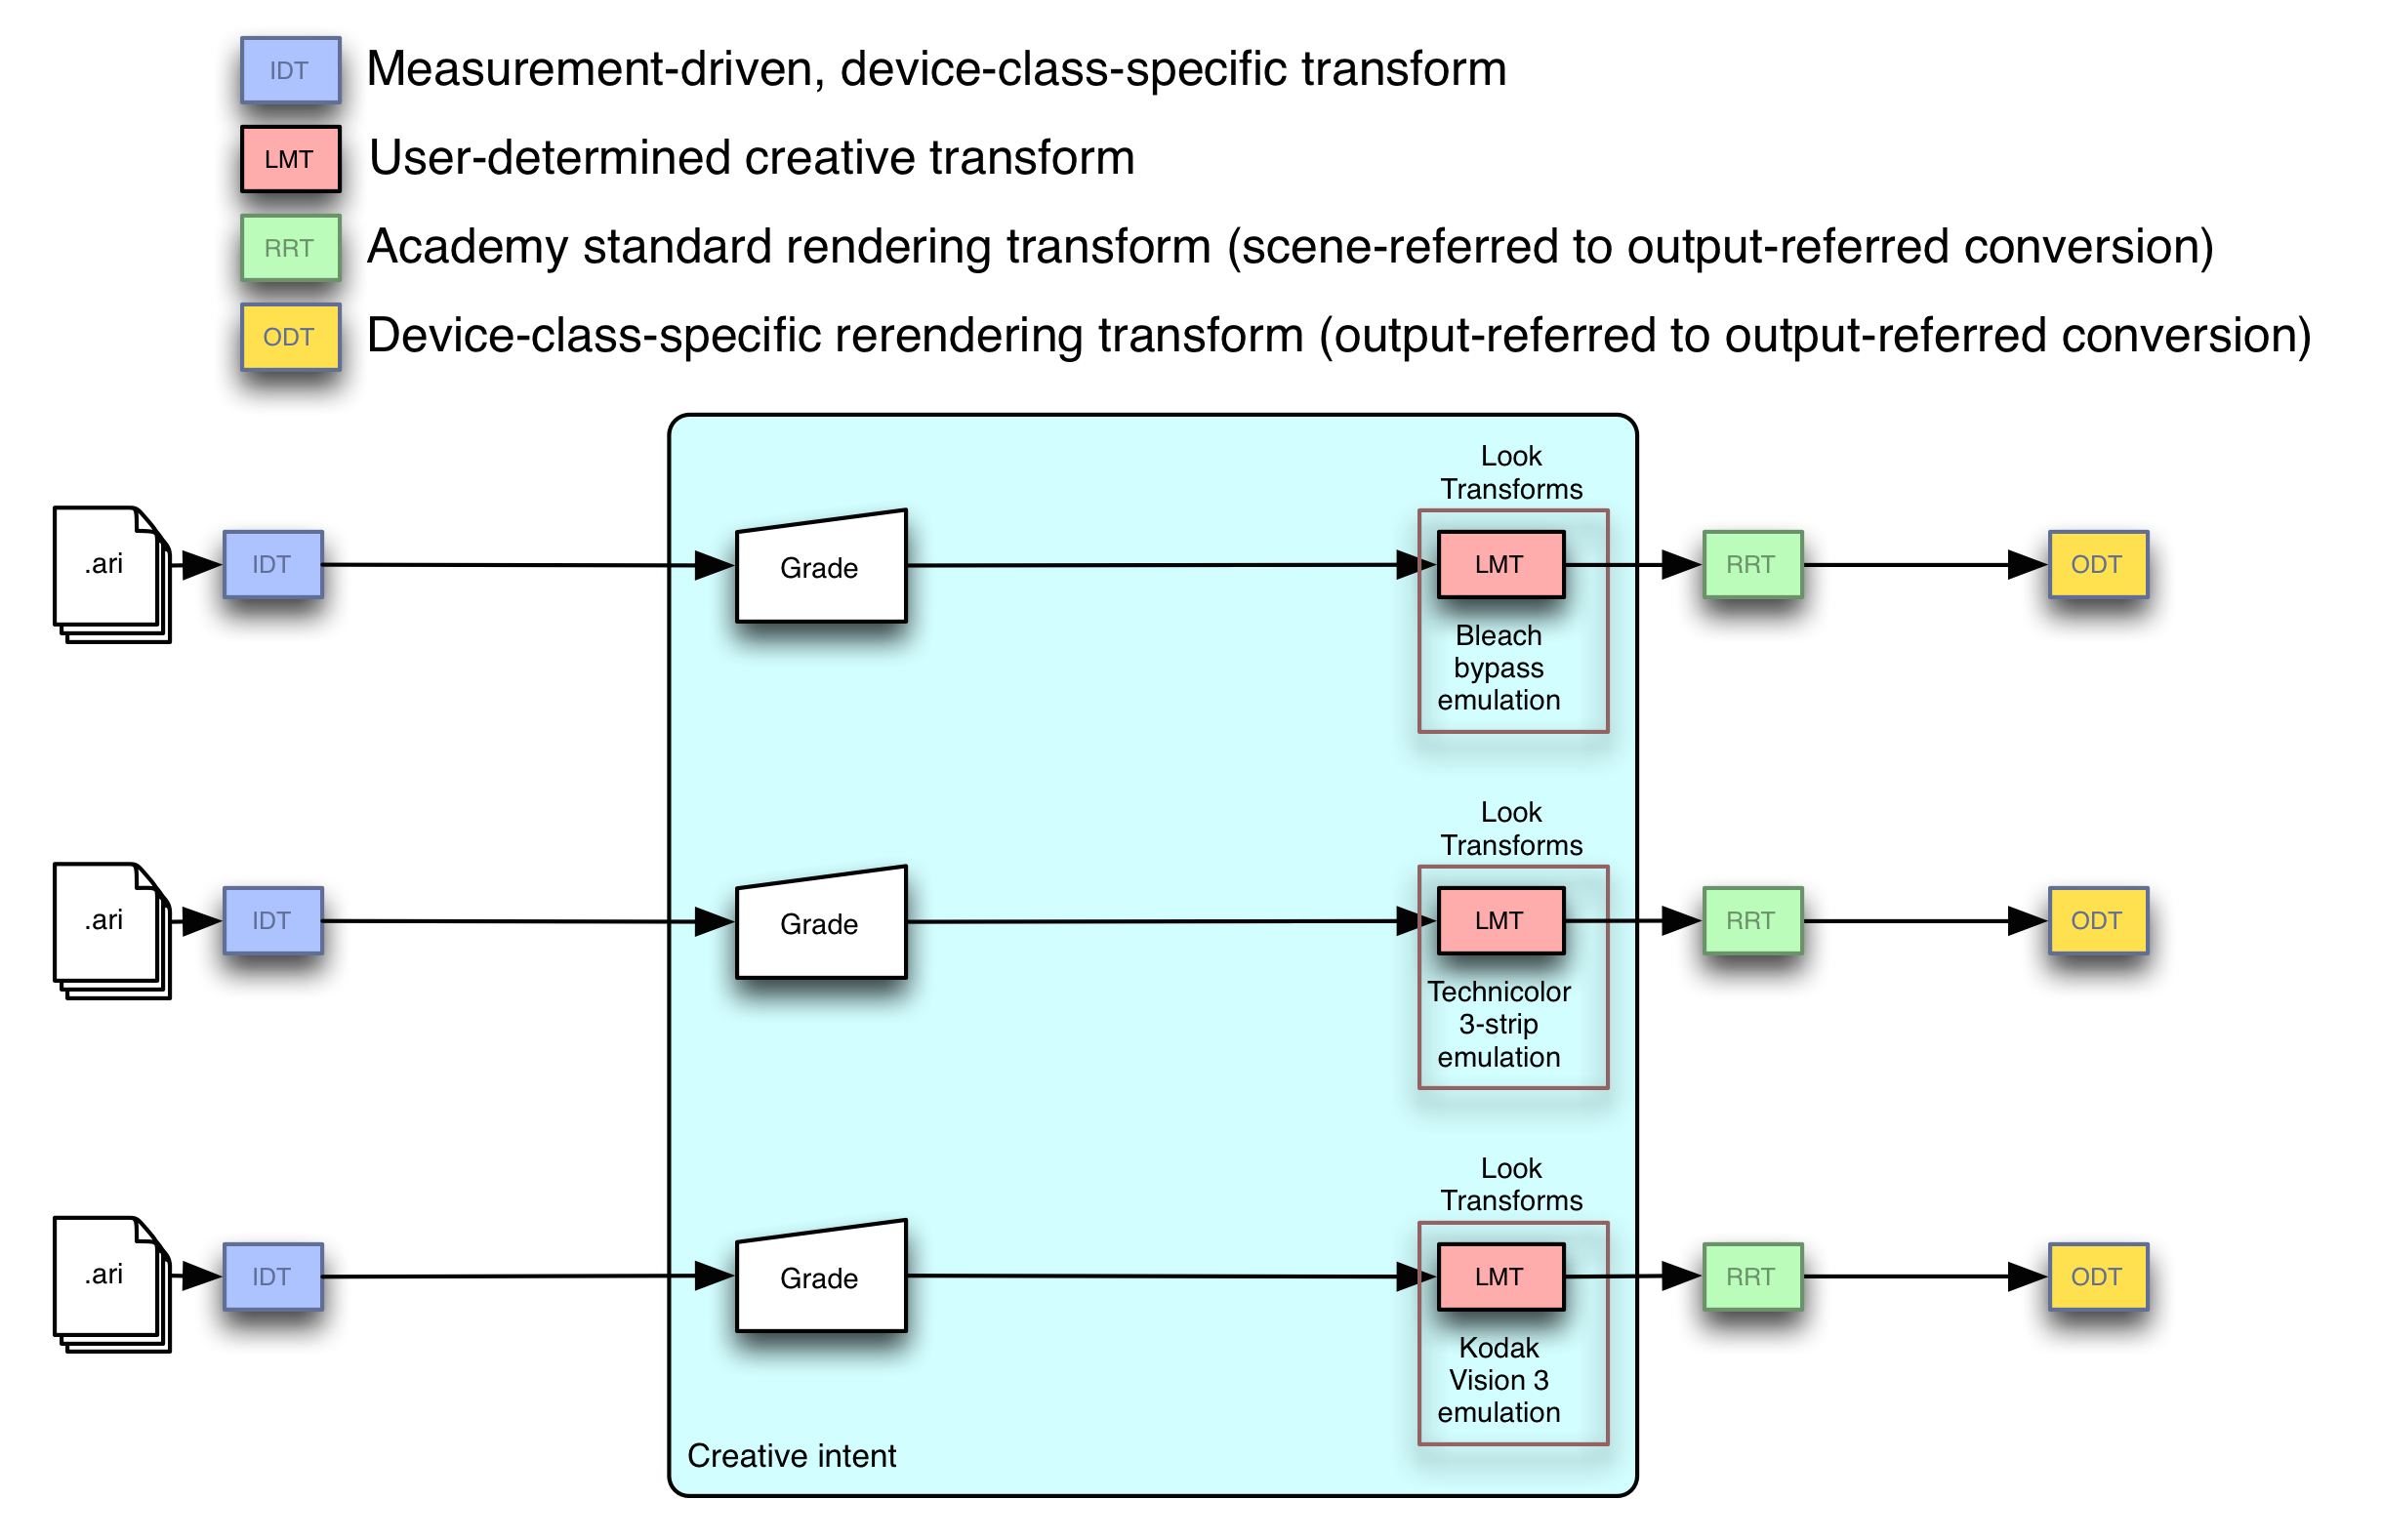
\includegraphics[width=\textwidth]{photochemicalProcessing.png}
\caption{}
\label{fig:photochemical}
\end{center}
\end{figure}

\section{Systematic Color Correction (and application of ASC CDL)}
The LMT takes as input an image in the ACES color space and yields a modified image that is still in the ACES color space. As a consequence, LMTs can be `chained' together, one after another. \autoref{fig:lmtChain} shows a grading workflow where, prior to applying the `Kodak Vision 3 emulation' LMT described above, the colorist applies an `ASC CDL' LMT—very likely one whose parameter values were chosen by the cinematographer on-set to modify the default `look' of emulated Kodak Vision 3 stock. 

\begin{figure}[H]
\begin{center}
    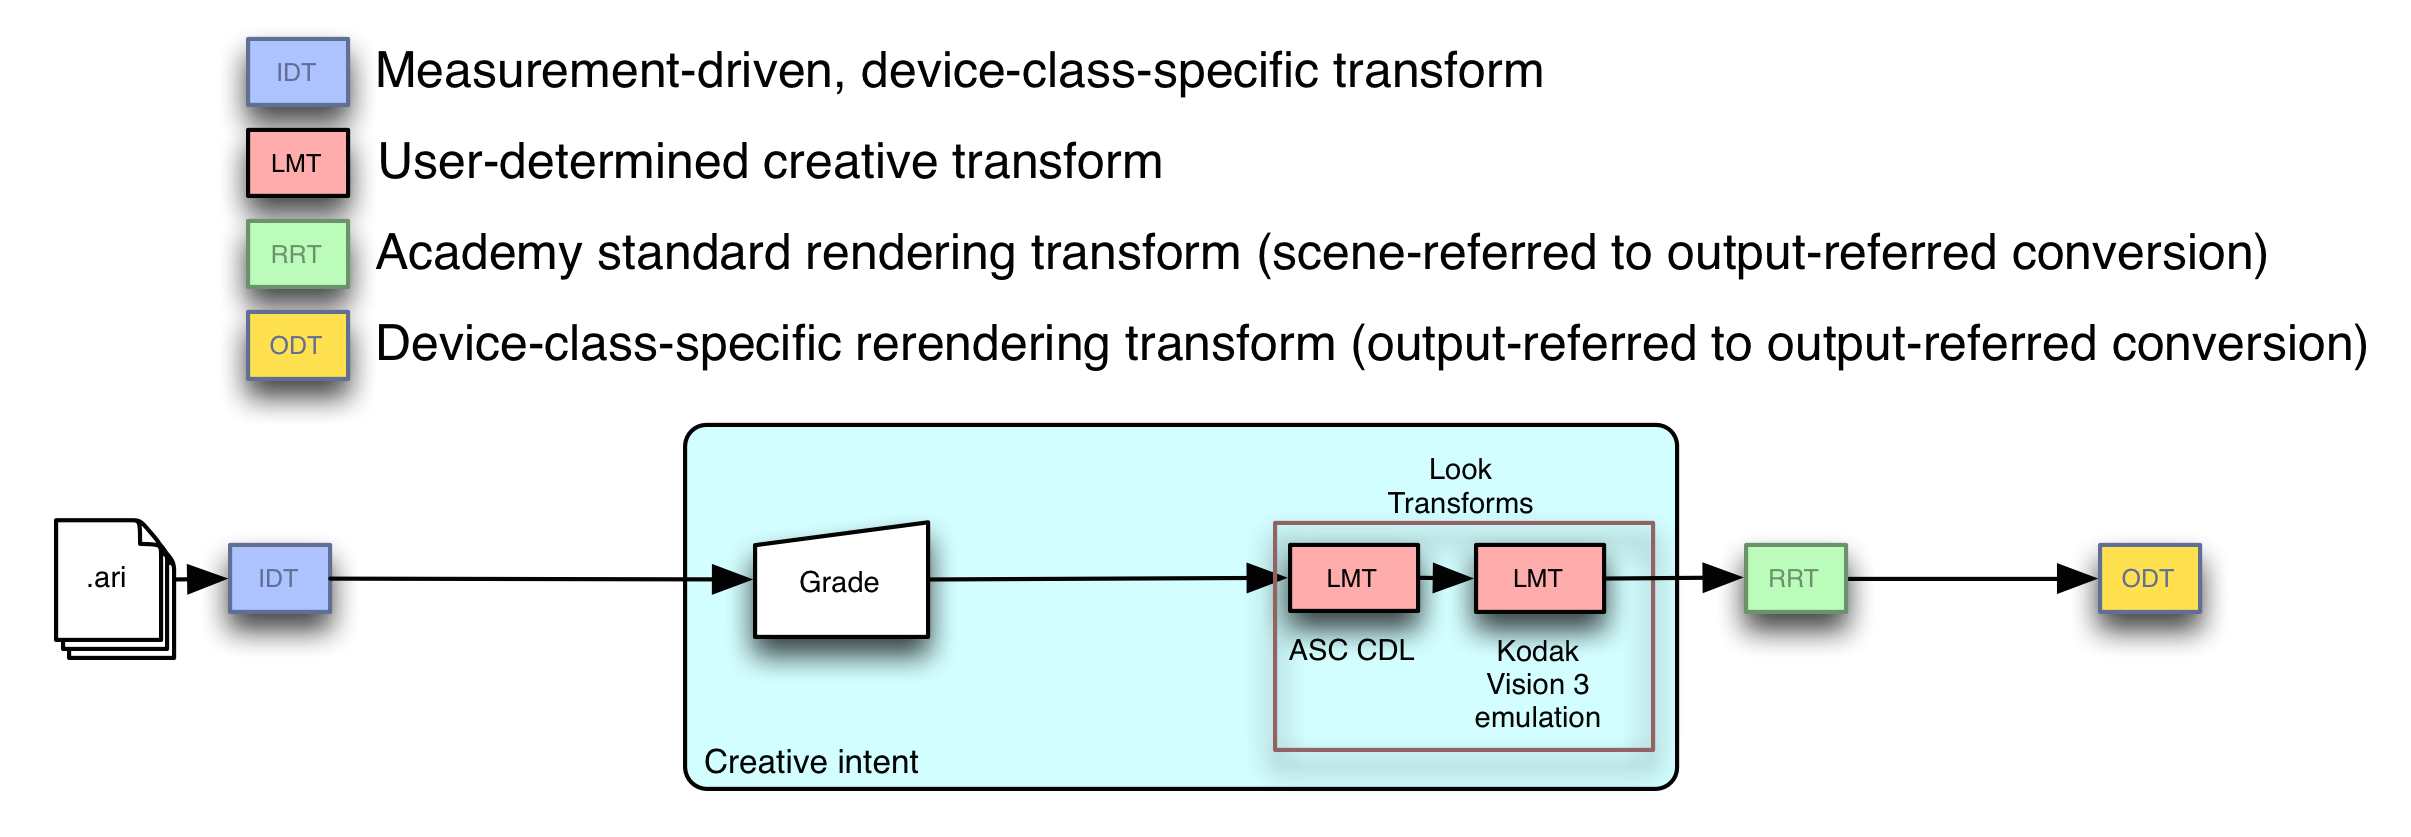
\includegraphics[width=\textwidth]{chainingLMTs.png}
\caption{}
\label{fig:lmtChain}
\end{center}
\end{figure}

\note{The values of the ASC CDL in this case are only valid in the context of the selected `Kodak Vision 3 emulation' LMT. If this LMT were removed, the ASC CDL values would no longer be valid.}
 
Note that the ASC CDL LMT incorporates a conversion from ACES to ACEScc before the ASC CDL operations will be applied, and likewise incorporates a conversion from ACEScc to ACES after the ASC CDL operations have been applied. This `wrapping' of ASC CDL operations is a key capability of the ACES Common LUT format.

\section{Trim Pass Grading}
Content today is delivered across a wide range of output devices, each of which has their own color space and characteristic brightness. Creative adjustments to the look of shots are often needed to enhance the content's appearance beyond the original creative intent. The client might desire to accentuate the difference between the results of the viewing pipeline for theatrical exhibition, the results of the viewing pipeline appropriate for home video and the results of the viewing pipeline appropriate for mobile streaming. This could be done by having three workflows that differed only in that the first had no LMT `accentuating' the image for any nonstandard viewing environment, the second had an LMT just prior to the application of the RRT and an ODT designated as appropriate for home video viewing, and the second had an LMT just prior to the application of the RRT and an ODT designated as appropriate for viewing with content streamed to mobile devices, as shown in \autoref{fig:trimPassGrading}.

\begin{figure}[H]
\begin{center}
    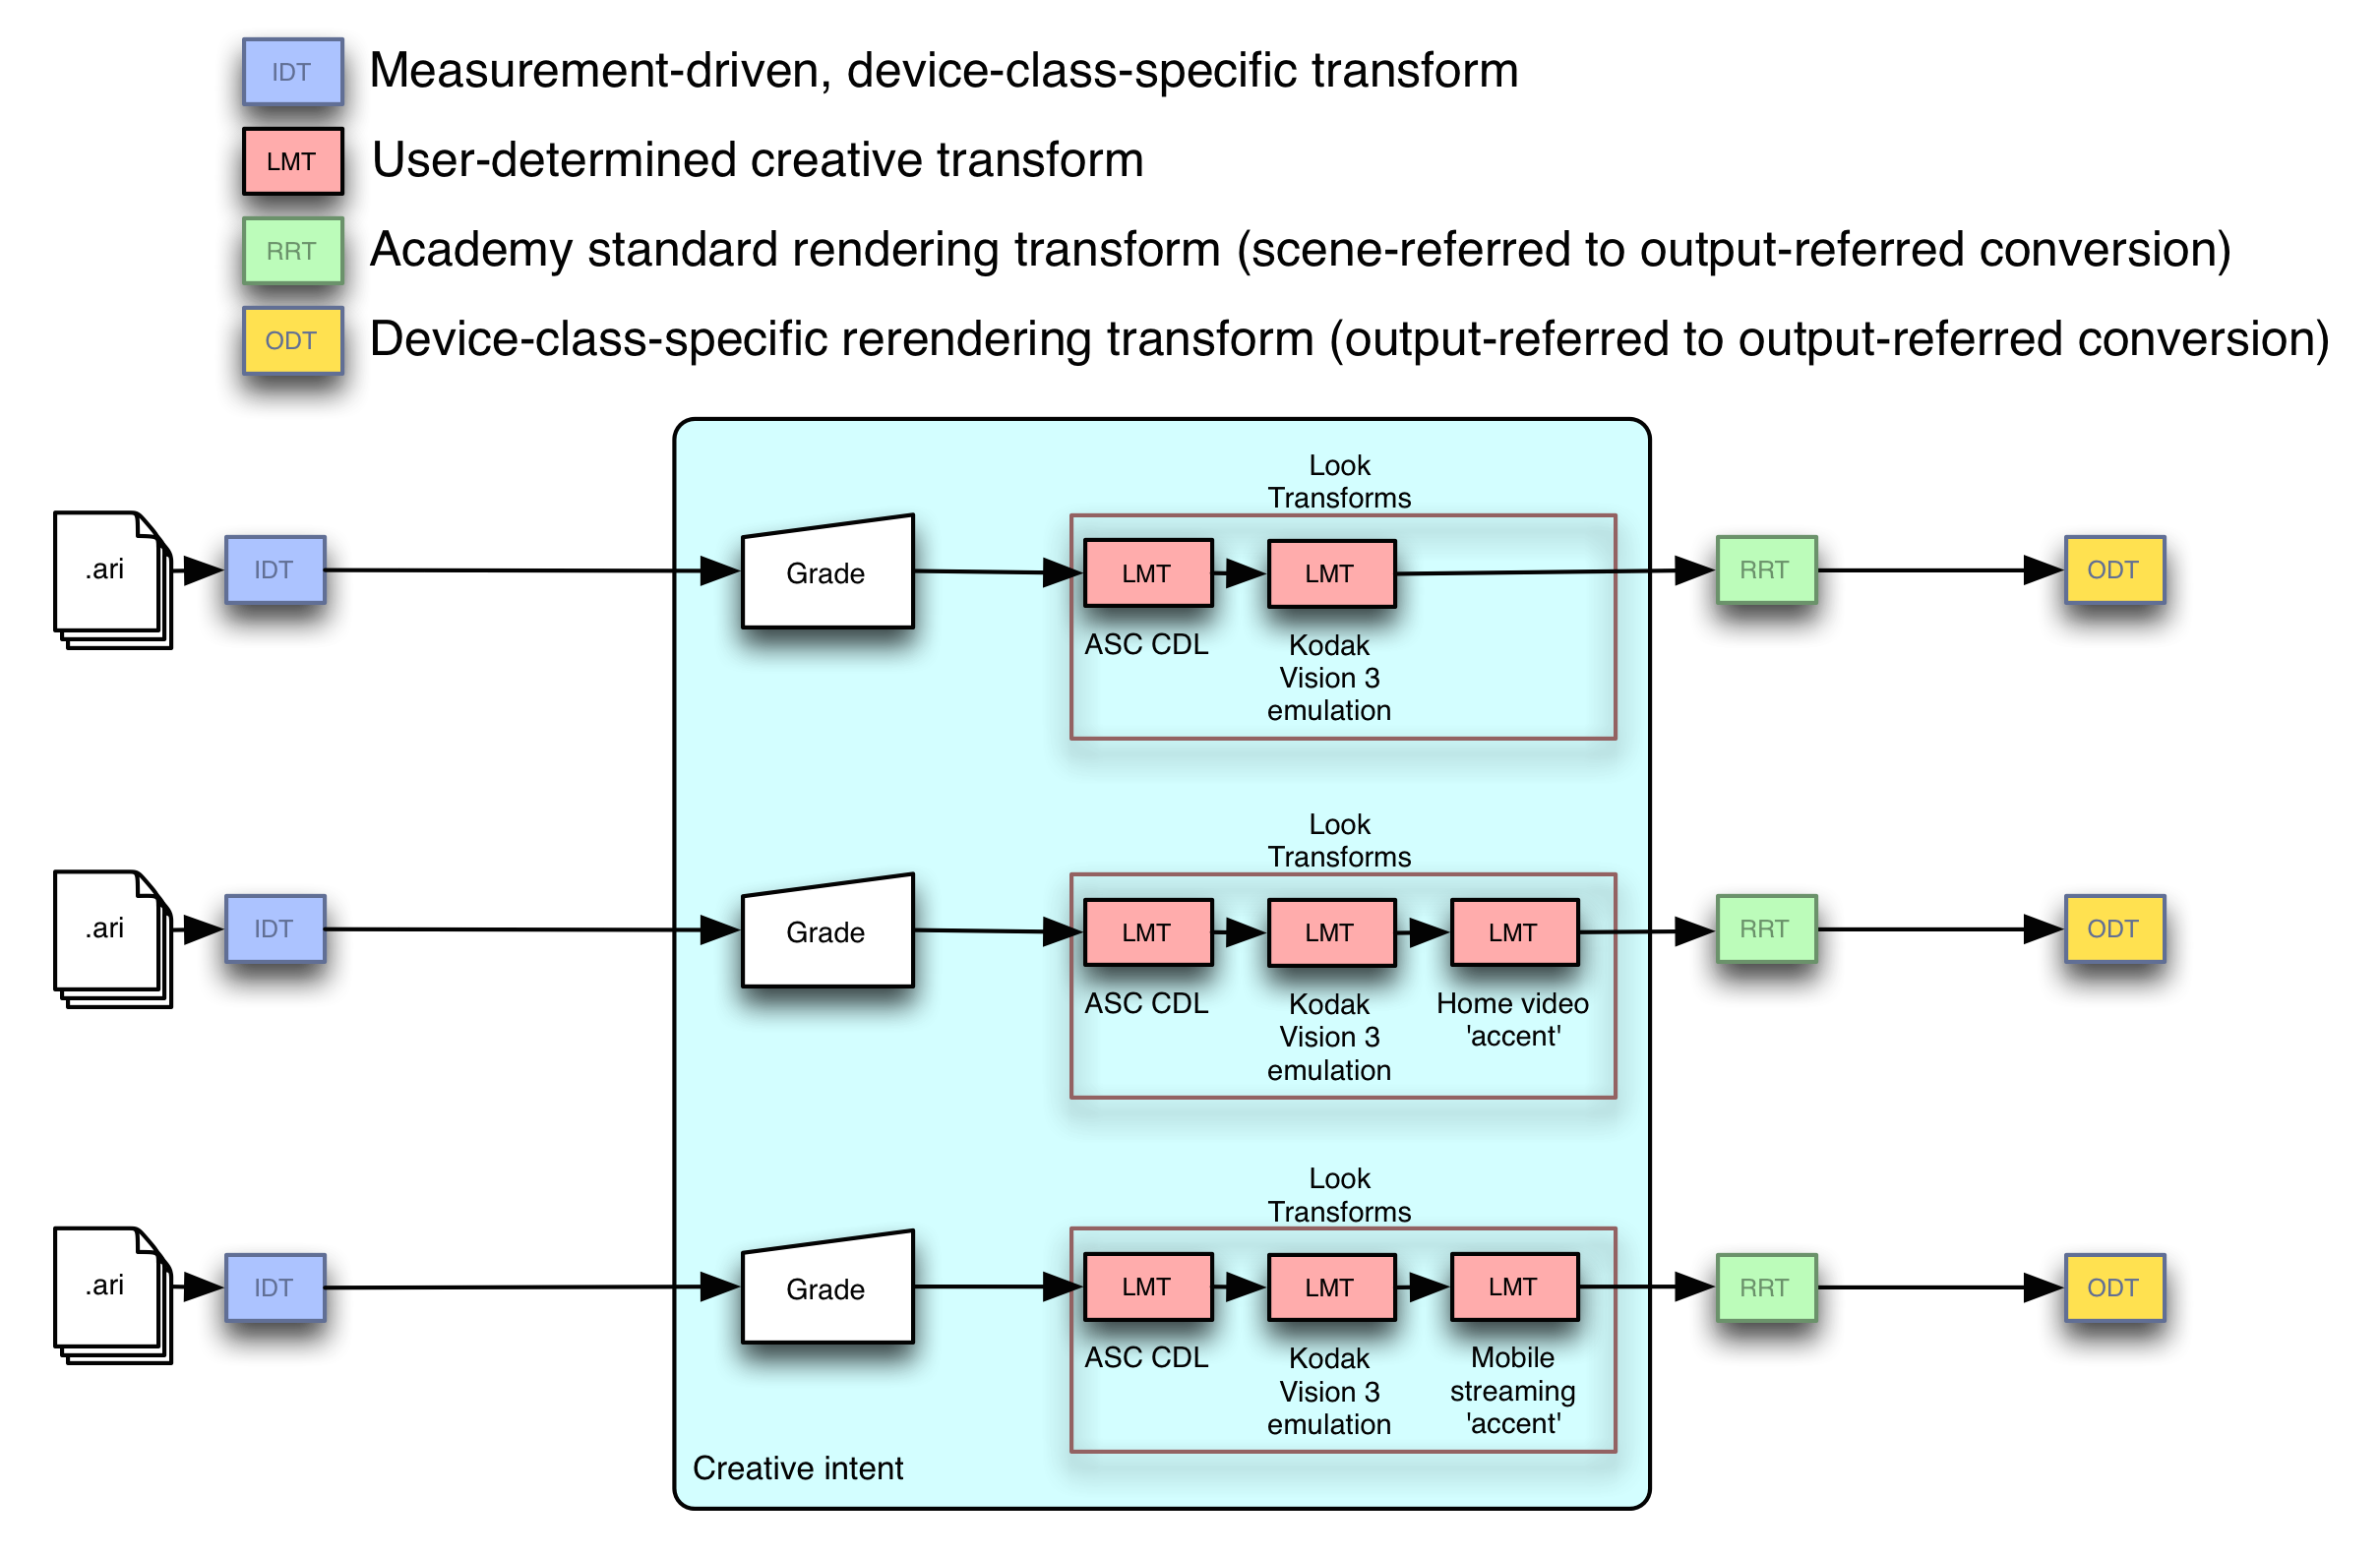
\includegraphics[width=\textwidth]{trimPassGrading.png}
\caption{}
\label{fig:trimPassGrading}
\end{center}
\end{figure}

\section{Flexible pre-sets for creative modifications}
Separation of grading and LMT(s) allows for a production to make significant changes in creative decisions that affect the entire frame equally, without requiring the colorist to start from scratch, or ideally without even requiring a trim pass. For example, the client might start a production shooting `day for night' and use an LMT to accomplish this result (\autoref{fig:dayForNight}).

\begin{figure}[H]
\begin{center}
    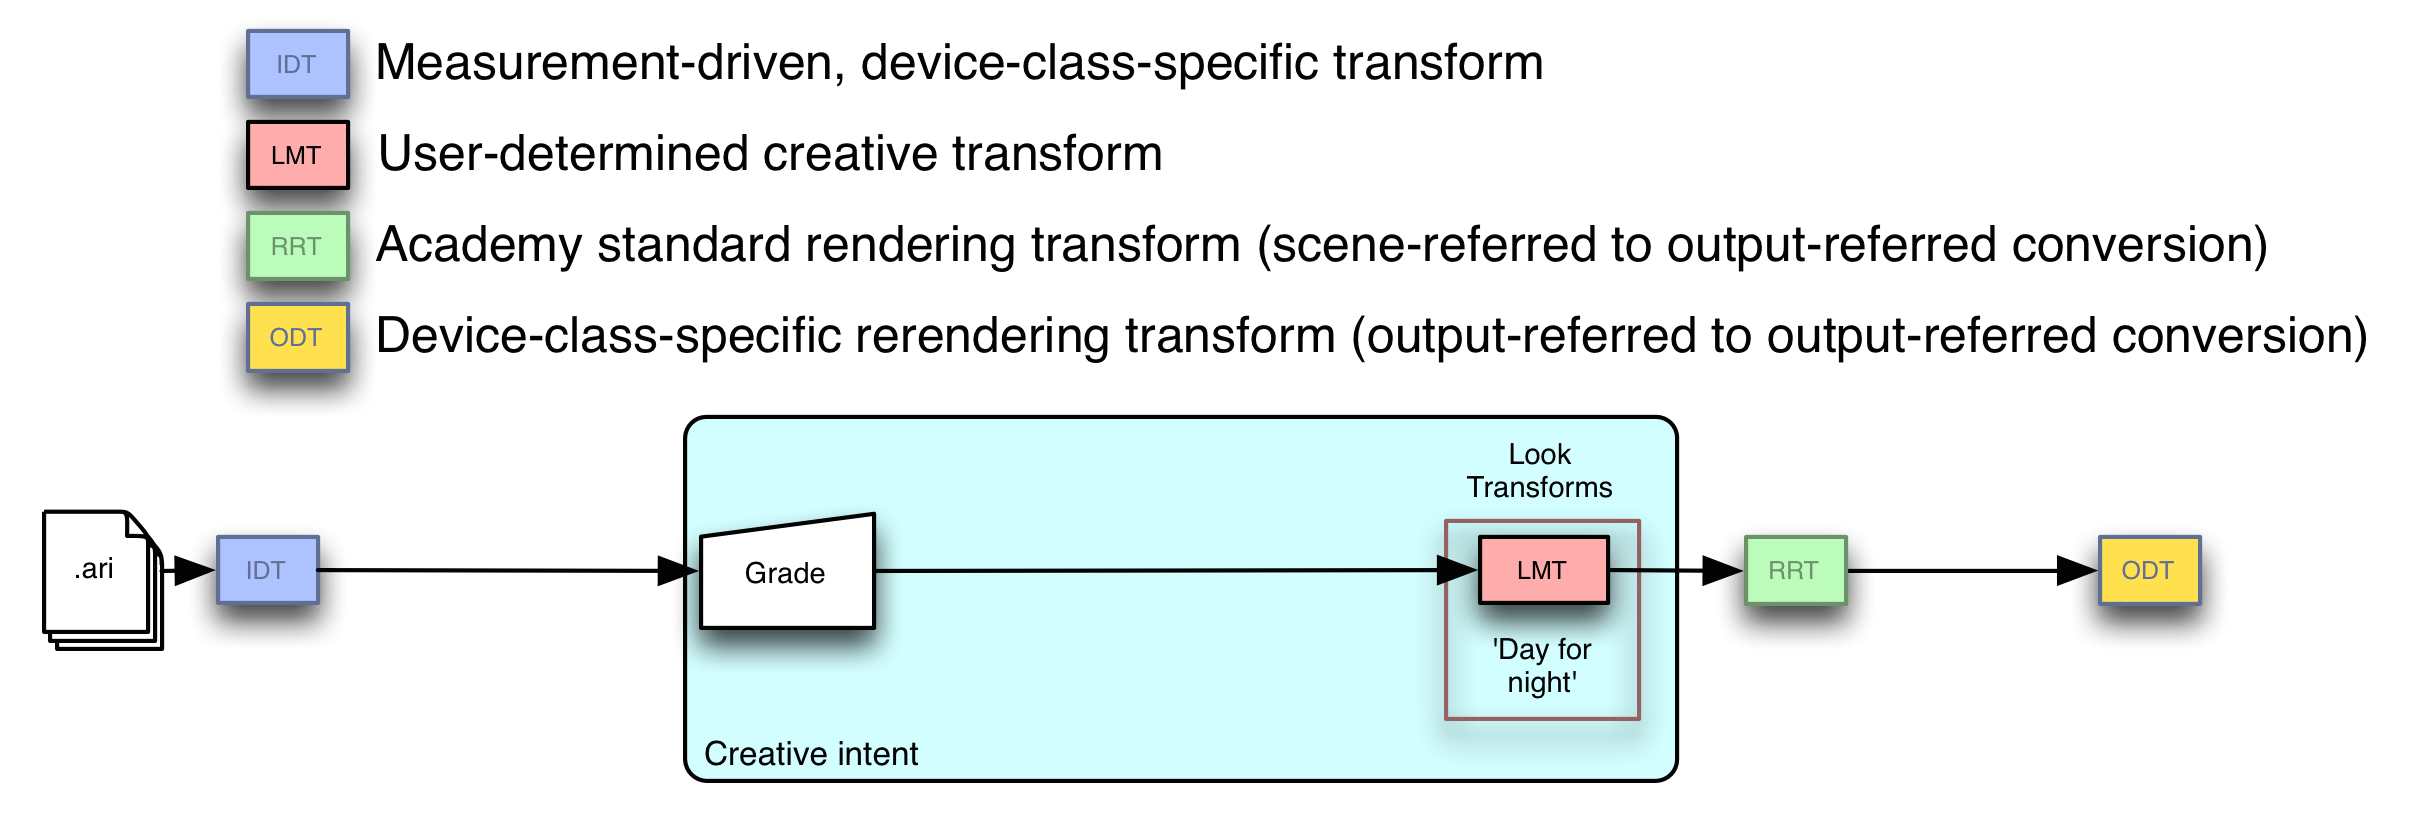
\includegraphics[width=\textwidth]{dayForNight.png}
\caption{}
\label{fig:dayForNight}
\end{center}
\end{figure}
 
A change in creative direction (say, after a test screening) might place the captured action two hours earlier, so `day for night' might become `day for dusk'. Since the LMT is separate from the grade, the change may be made without requiring lengthy and expensive colorist intervention. A new LMT is simply swapped into the old LMT's place (\autoref{fig:dayForDusk}).

\begin{figure}[H]
\begin{center}
    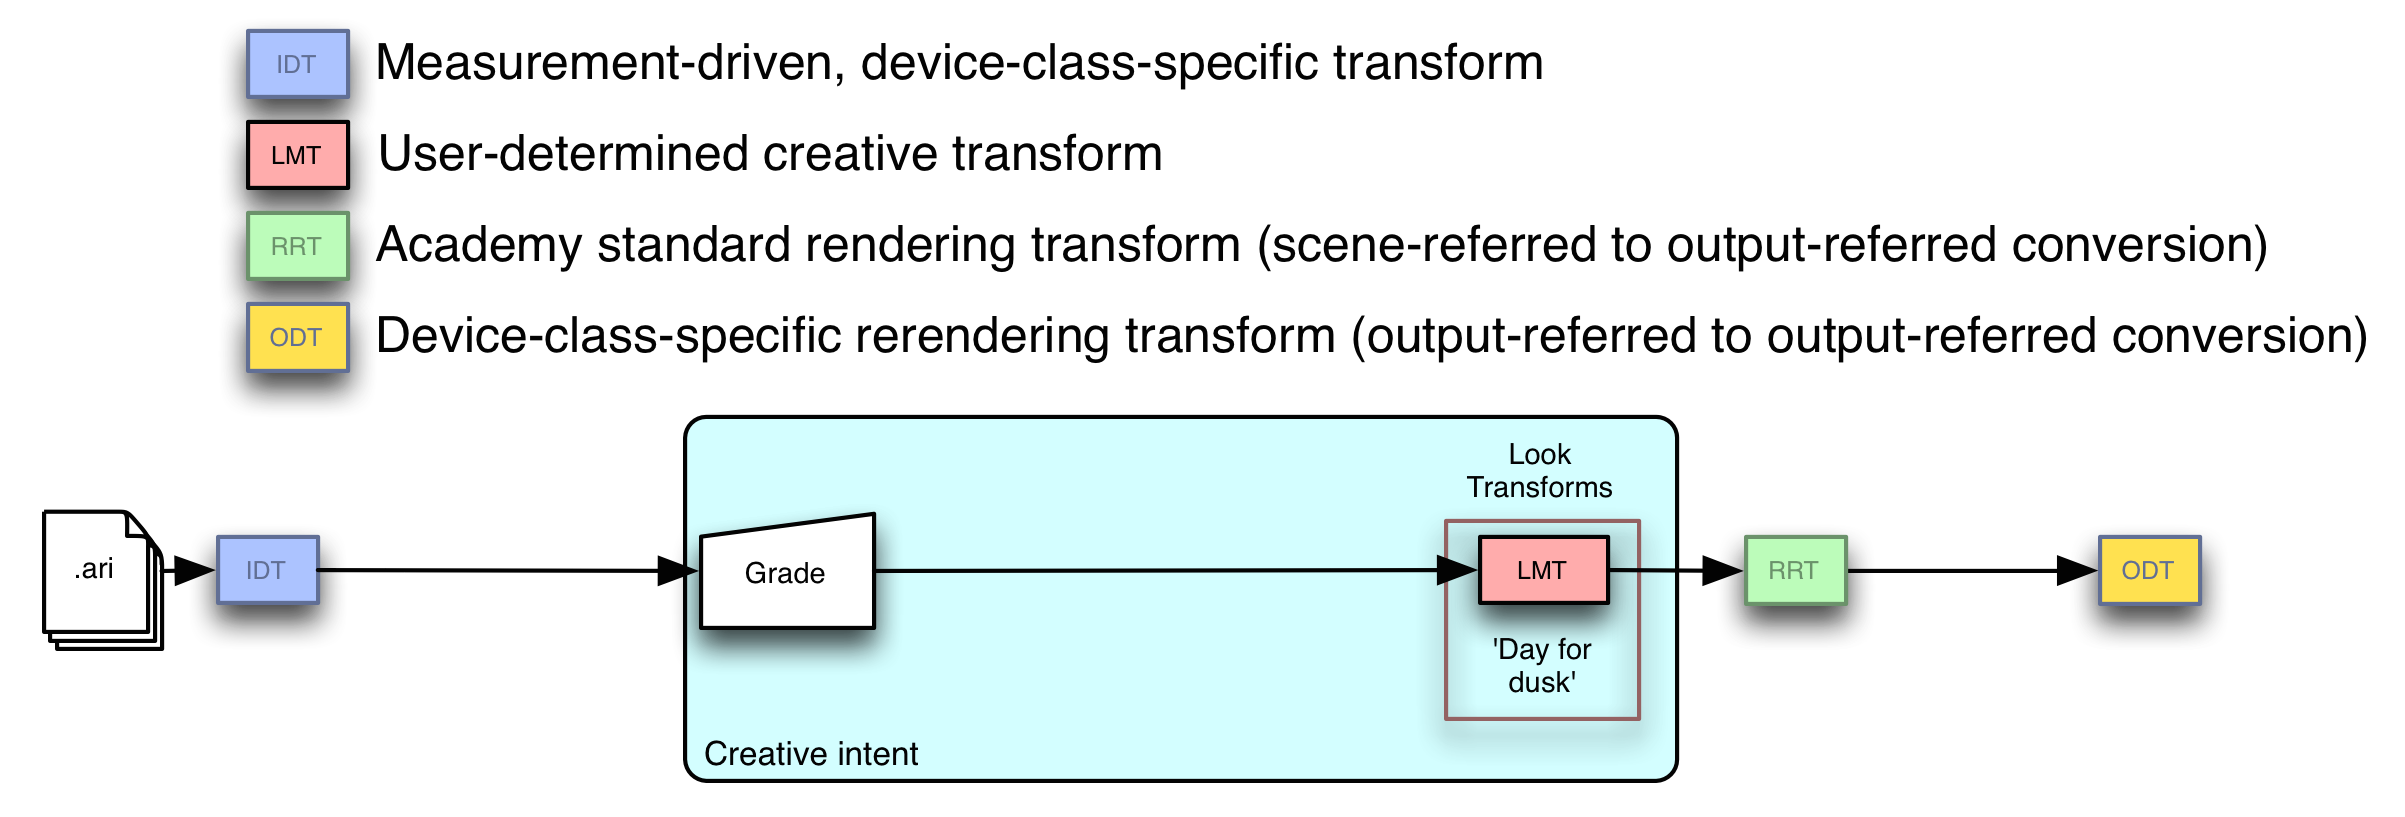
\includegraphics[width=\textwidth]{dayForDusk.png}
\caption{}
\label{fig:dayForDusk}
\end{center}
\end{figure}

\section{Permanent Color Modification (archival)}
The workflows above all show a `transient' processing of image file to displayed output, with the display being a calibrated grading monitor or projector. It is also completely valid and correct to archive the input to the RRT as an ACES container file, `baking in' the grade and any LMT application(s), as shown in \autoref{fig:archival}.

\begin{figure}[H]
\begin{center}
    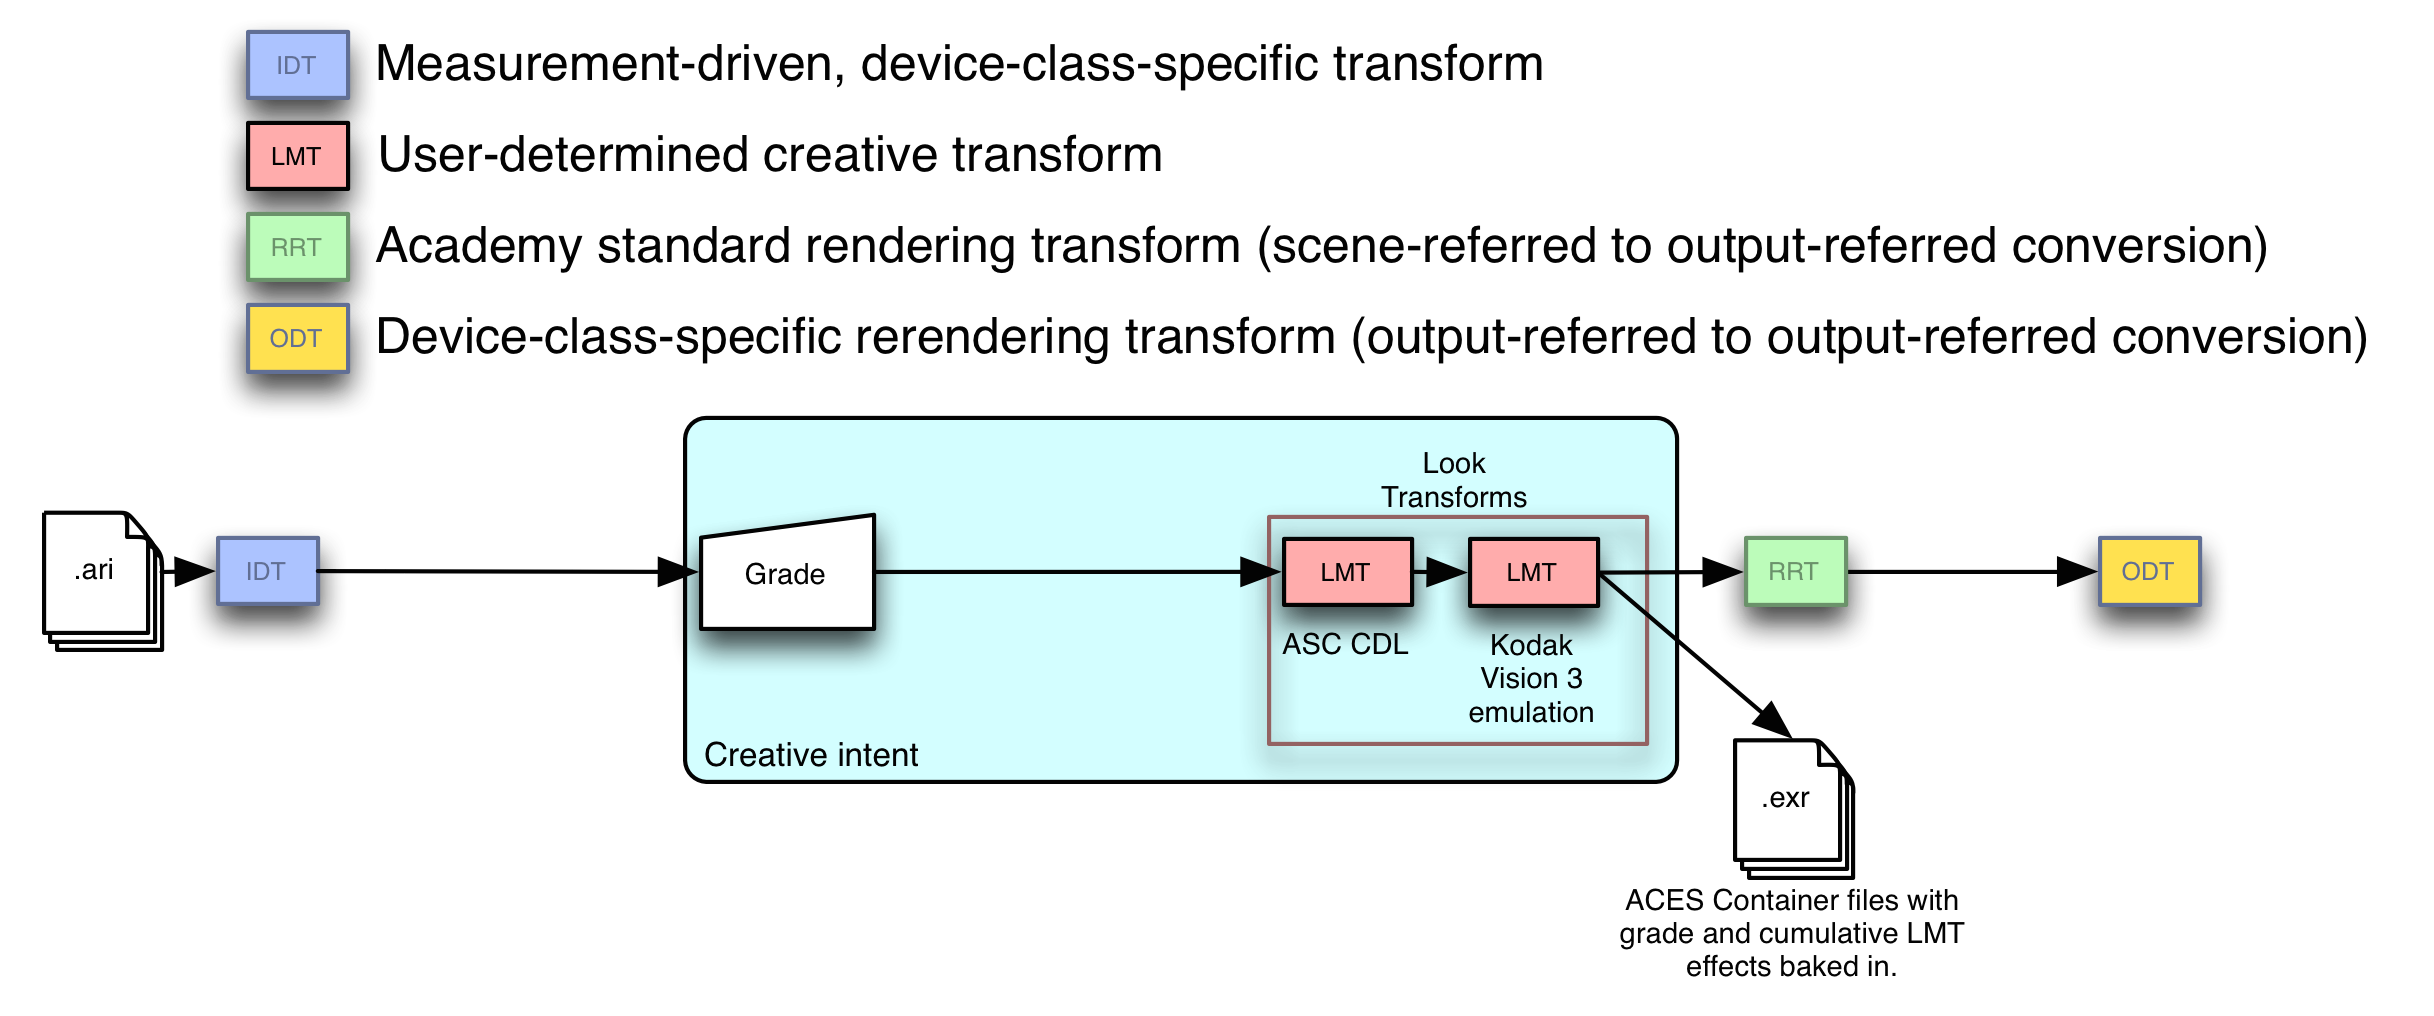
\includegraphics[width=\textwidth]{archival.png}
\caption{}
\label{fig:archival}
\end{center}
\end{figure}

A person who retrieves an ACES file need not know about the grades and LMT(s) applied to produce the desired creative result; by virtue of being an ACES file, the image `speaks for itself' when the RRT and a selected ODT are applied. 

It is extremely important that the LMT authors preserve as much of the dynamic range of the LMT’s input ACES RGB relative exposure values as is possible. This provides the maximum amount of latitude for a colorist grading through the LMT. It also preserves the maximum amount of grading latitude for someone who later retrieves stored ACES container files created by ‘baking in’ the effect of the LMT to the graded ACES images, when remastering for a radically different display or viewing environment (e.g. for grading on a higher-dynamic-range display than previously available). While full preservation of dynamic range and gamut is almost never possible, when faced with an engineering decision in which all other considerations are equal, the LMT author should choose the option that retains more of the LMT input’s dynamic range and color gamut.

Preserving the integrity of the ACES RGB relative exposure values representing the scene means more than just not clipping highlight luminances or very deep shadow tones. It also means avoiding severe distortions of the distributions of ACES values, such as the distortion caused by a strong `gamma' operation, e.g. by a very large or very small value for one or more CDL `power' parameters.

Because LMT's are customizable and unique, and because it is essential to maintain the portability and archivability of an ACES project, it is always necessary to preserve the LMT transforms within any project where they are used.

\note{If a production wishes to preserve maximum flexibility for later remastering, it should archive the original ACES images, any clip-level metadata-bearing container encapsulating the original image files, any IDT(s), any pre-grading adjustments (see the following `LMTs and pre-grading for Visual Effects' section), any project-wide and shot-specific grading parameters, and the Look Transform (that is, the set of all LMTs employed to achieve the creative result, in their proper sequence).}

\section{Portability}
LMTs are expressed and transported using the Common LUT format (also known as the Academy/ASC LUT format or the ASC/Academy LUT format).

The building blocks of an LMT include basic arithmetical operations, simple matrix application, 1D LUTs and 3D LUTs. Straightforward color transforms can often be expressed analytically using the first three of these building blocks. More complex (and typically empirically derived) LMTs may be conveyed as 3D LUTs. The Common LUT format was chosen because it can express, in a portable encoding, all of the abovementioned operations and LUTs.

\note{Using the floating point ACES RGB relative exposure values directly as 1D LUT indices requires a more complex lookup mechanism than found in traditional 1D LUT implementations. The Common LUT Format supports this type of lookup by using the halfDomain attribute of the LUT1D process node; see the Common LUT Format documentation for more information.}

\section{LMTs and pre-grading for Visual Effects}
In some cases, color corrections may be created prior to the colorist session in a scene-balancing `pre-grade.' This allows for all shots in a sequence to share identical LMTs `downstream' in the color modification pipeline. A motivating case would be a long sequence of daylight shots with varying color temperature.
An example of this workflow, with two illustrations, is shown below. The first illustration shows what might happen at a visual effects facility that receives a number of shots that will be edited together to make up a sequence.

\begin{figure}[H]
\begin{center}
    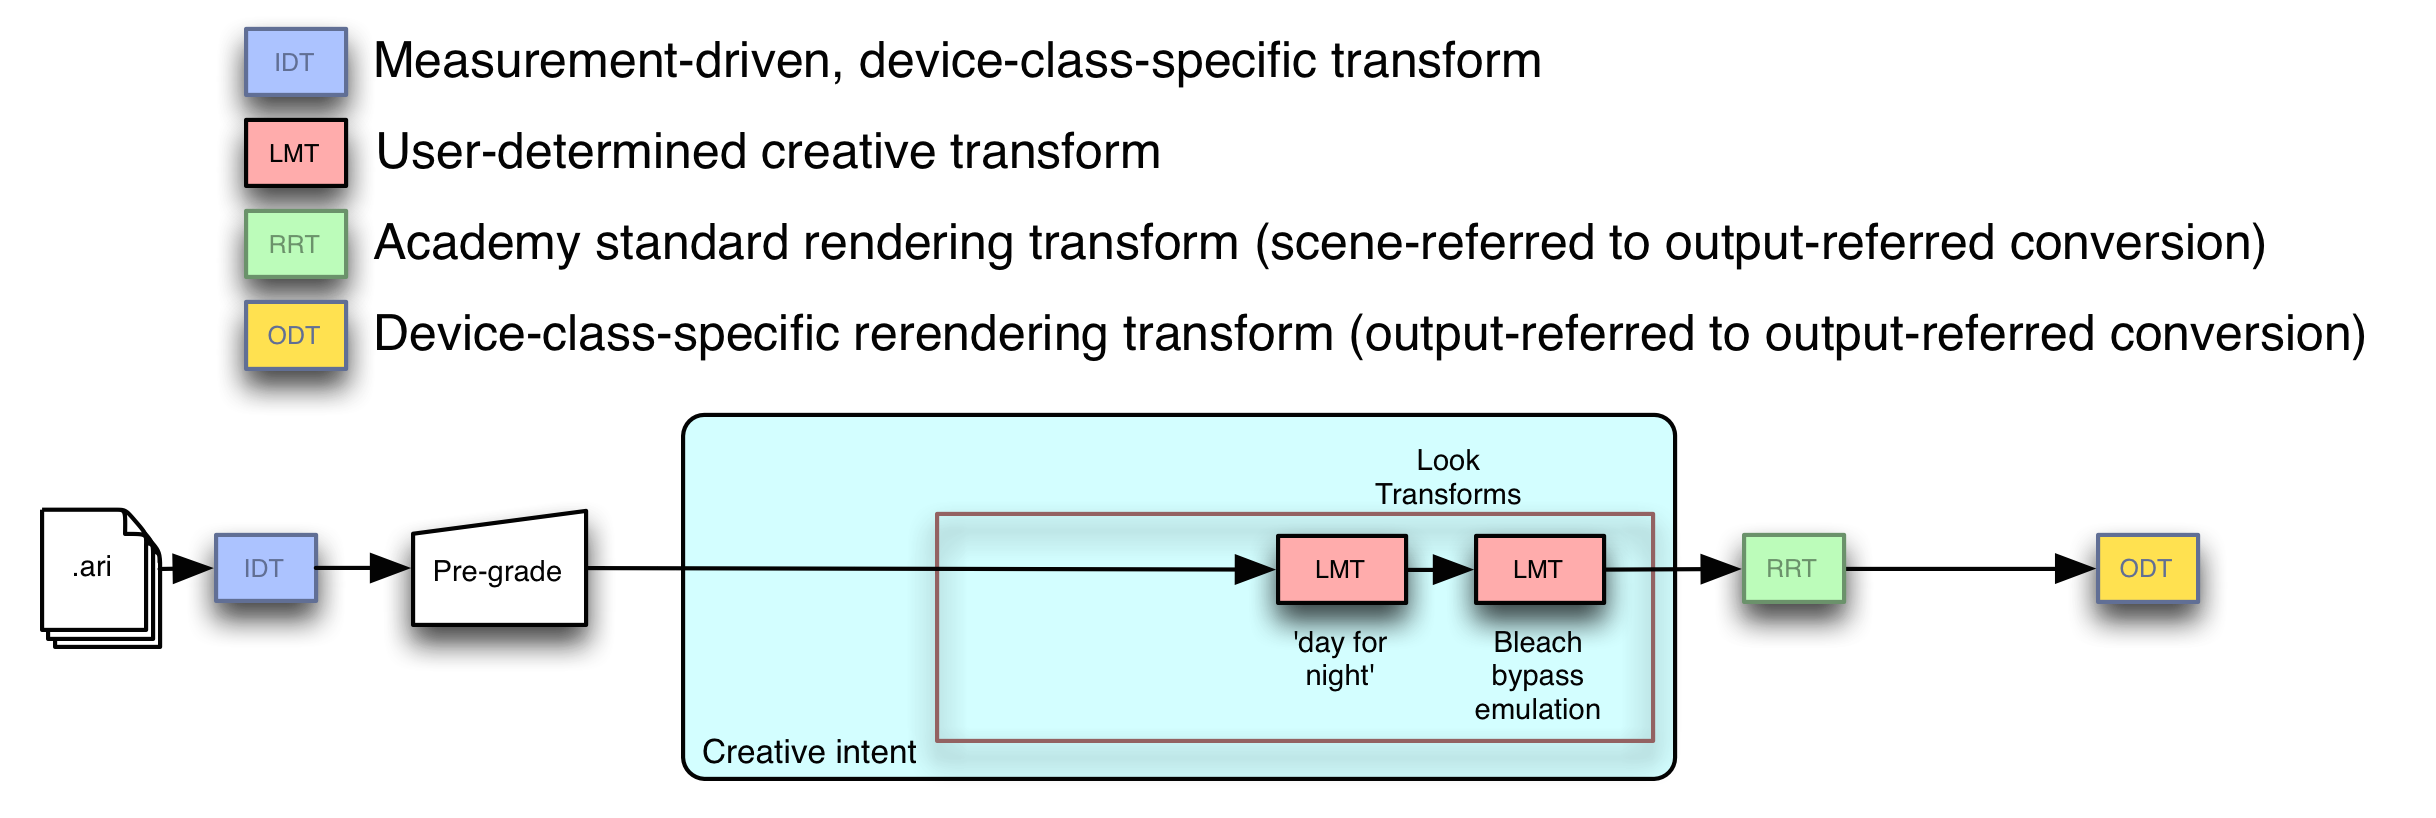
\includegraphics[width=\textwidth]{vfx1.png}
\caption{}
\label{fig:vfx1}
\end{center}
\end{figure}

When the visual effects are complete, the frames supplied to the colorist have both the pre-grade and the visual effect(s) `baked in.' The Look Transform is not `baked in' to this imagery, since it must be applied after the grade, but is instead carried as metadata, and is referenced by the ACES clip container.

\begin{figure}[H]
\begin{center}
    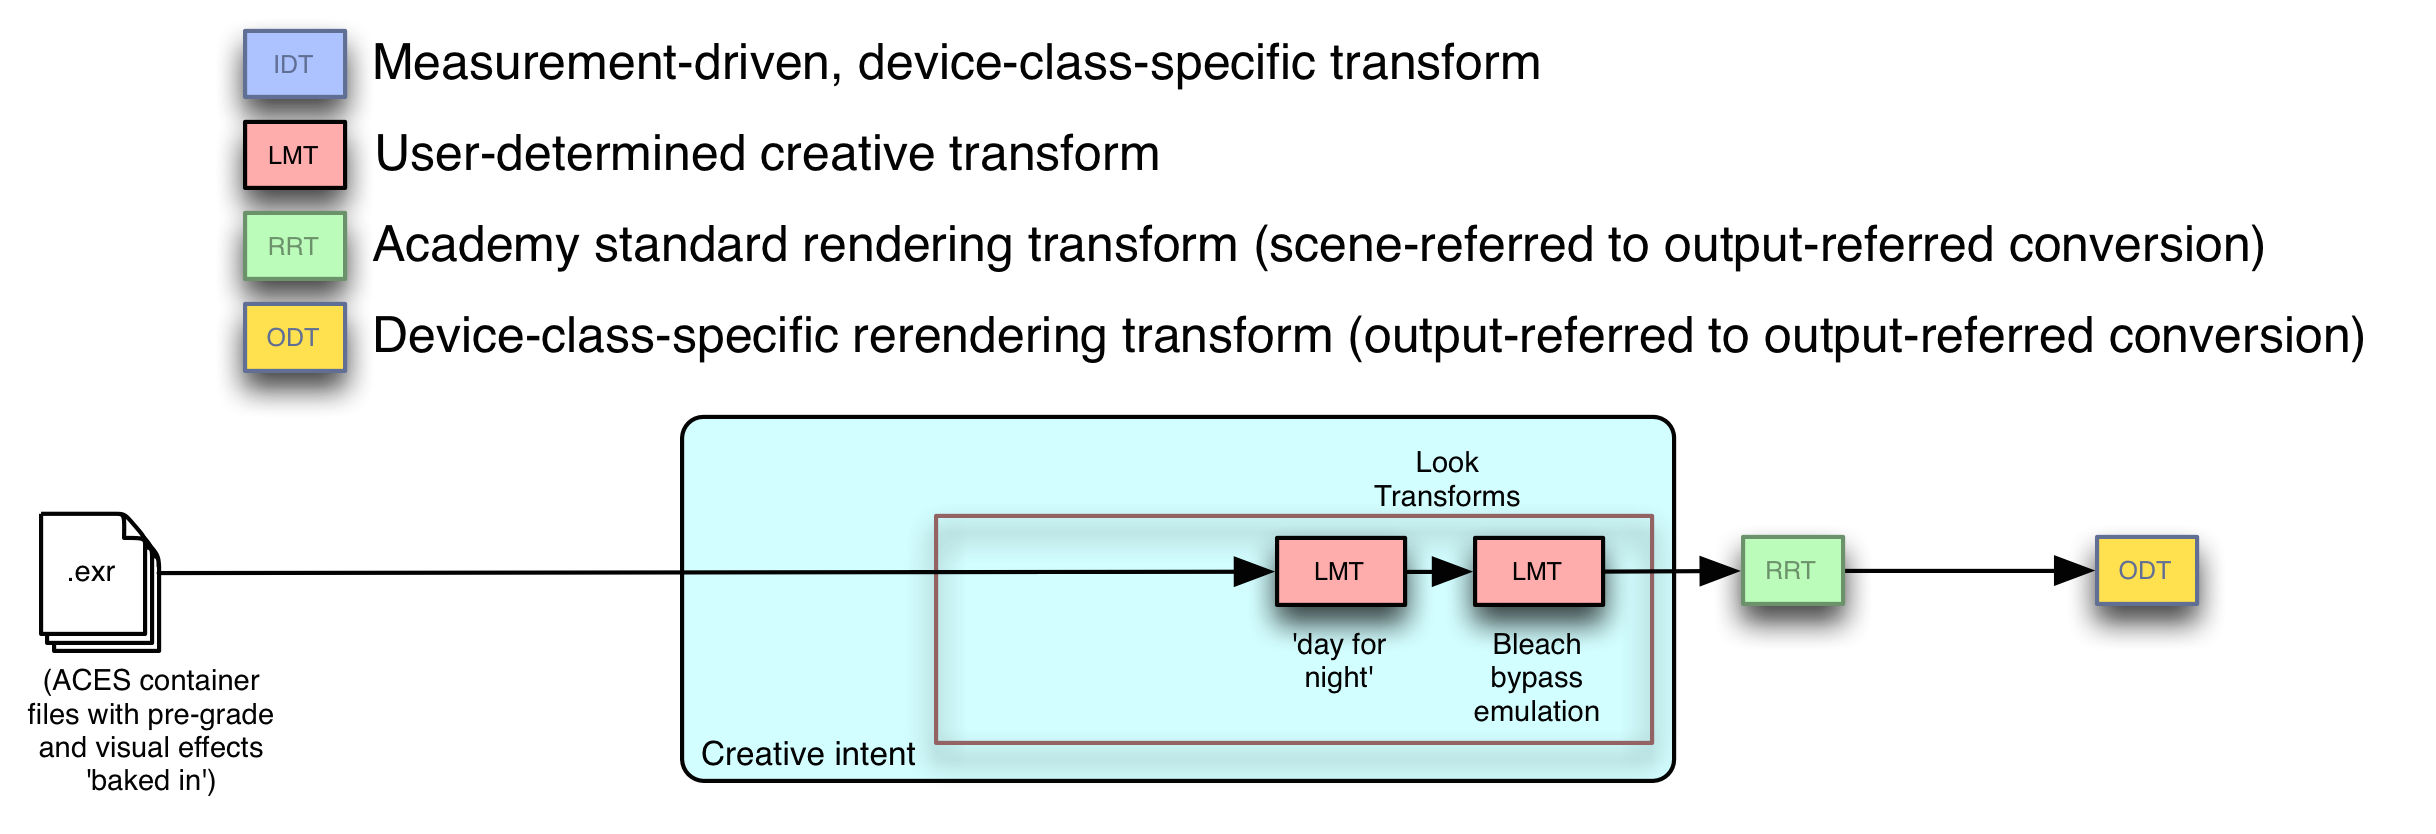
\includegraphics[width=\textwidth]{vfx2.png}
\caption{}
\label{fig:vfx2}
\end{center}
\end{figure}


% This file contains the content for a main section
\regularsectionformat
%% Modify below this line %%
\chapter{Versioning System Specification}
In the following definitions, \textit{italics} represent a changeable placeholder. \textbf{boldface} represents a required string or character.

\section{String Formats}
ACES system components shall use the following versioning string formats where applicable:

\texttt{\textit{Type.}\textbf{a}\textit{MajorVersionNumber.MinorVersionNumber.PatchVersionNumber}}

or

\texttt{\textit{Type.Name.}\textbf{a}\textit{MajorVersionNumber.MinorVersionNumber.PatchVersionNumber}}

where \texttt{Type} is one of the following:

\begin{listize}
    \item \texttt{ACES2065-1} -- Academy Color Encoding Specification, SMPTE 2065-1
    \item \texttt{ACESrelease} -- ACES system release version
    \item \texttt{ACEScc} -- ACES color grading working space
    \item \texttt{ACESproxy} -- ACES ``wire format''
    \item \texttt{ACEScg} -- ACES CG/VFX working space
    \item \texttt{ADX} -- Academy Density Exchange Specification, SMPTE 2065-3
    \item \texttt{IDT} -- ACES Input Transform (a.k.a. ``Input Device Transform'')
    \item \texttt{LMT} -- ACES Look Transform (a.k.a. ``Look Modification Transform'')
    \item \texttt{ODT} -- Output Device Transform
    \item \texttt{RRT} -- Reference Rendering Transform
    \item \texttt{RRTODT} -- ACES Output Transform (concatenated RRT and ODT)
    \item \texttt{InvRRT} -- Inverse Reference Rendering Transform
    \item \texttt{InvODT} -- Inverse Output Device Transform
    \item \texttt{InvRRTODT} -- ACES inverse Output Transform (concatenated RRT and ODT)
    \item \texttt{ACESlib} -- ACES library functions for core transforms, e.g., Tonescales
    \item \texttt{ACEScsc} -- ACES color space conversion transforms
    \item \texttt{ACESutil} -- utility functions provided with the ACES release, e.g., Adjust_Exposure
\end{listize}

ACES system components are assigned a string that serves as a unique identifier for an ACES System Release. This identifier is constructed using a set of tokens as described in this specification so that it will be more human-readable than a typical Universally Unique Identifier (UUID).

If the \texttt{PatchVersionNumber} is zero, it may be omitted from the versioning string for simplification. If both the \texttt{MinorVersionNumber} and the \texttt{PatchVersionNumber} are zero, they may both be omitted from the versioning string for simplification.

\section{ACES Transform Identifiers}
ACES transforms, expressed as CTL files, are assigned a Transform Identifier.  The Transform Identifier shall be included with all Product Partner implementations intended to match that ACES transform. The Transform Identifier shall be contained in the transform files as metadata or as a comment. For Academy-supplied transforms, the Transform Identifier plus an extension shall be used for the file name. The extension (e.g. .ctl) is not considered part of the Transform Identifier.

Product Partner implementation transforms may be intended to match the results of a combined series of ACES CTL transforms, e.g., LMT+RRT+ODT.  In that case, all of the relevant ACES Transform Identifiers shall be included in the implementation Transform. The RRT+ODT combination is a unique case that is covered in \autoref{sec:rrtodt} below.

\section{Friendly Names}
ACES Transform Identifiers can be complex and therefore not appropriate for presentation to end users for selection purposes. All transforms should include ``friendly names'' as metadata within the transform file that software applications may access them for presentation in their user interfaces. Recommended friendly names are described in a separate document, ``Academy TB-2014-002, ACES Version 1.0 User Experience Guidelines.''

\section{ACES System Release}
The ACES System Release consists of a variety of ACES core components and ACES vendor-supplied components.

The ACES System Release version shall use the following versioning convention: 

\texttt{\textbf{ACESrelease.a}\textit{MajorVersionNumber.MinorVersionNumber.PatchVersionNumber}}

The ACES System Release major version number shall be incremented with substantive changes to the ACES core components. When the ACES System Release major version number is changed it will require all core and vendor-supplied components be updated to confirm compatibility with the new ACES major version.

The ACES System Release minor version number shall be incremented with non-substantive changes, e.g., a roll-up of minor ODT enhancements/additions or bug fixes. New ACES System Release minor versions shall not require an update to all ACES core and vendor-supplied components.

The ACES System Release patch version number shall be incremented with bug fixes. New patch versions shall not require an update to all transforms.

The ACES System Release version will not be incremented when ACES vendor-supplied components are updated.

\section{ACES Core Components}
ACES core components include: 

\begin{listize}[-]
	\item ACES Core Transforms
	\item ACES Core Encodings
	\item ACES Core Libraries and Utilities
	\item ACES Core File Formats
\end{listize}

\subsection{ACES Core Transforms}
The ACES Core Transforms include the following:

\begin{listize}[-]
	\item The Reference Rendering Transform
	\item Academy-supplied Output Device Transforms
	\item Academy-supplied Look Modification Transforms
\end{listize}

Transforms such as the RRT and ODTs rely on sub-functions included in separate CTL files (ACESlib). Whenever a change is made to the code of a sub-function, the version of the Transform Identifier will be incremented (even if the code in the RRT, ODT, etc. itself may not have changed). Since the results of an ODT depend on the RRT, whenever the RRT version is incremented, the version of all ODTs will also be incremented.

\subsubsection{Reference Rendering Transform (RRT)}
The RRT major version number shall match the ACES System Version Major Version number. The RRT Transform Identifier shall use the following versioning convention:

\texttt{\textbf{RRT.a}\textit{ACESmajorVersionNumber.RRTminorVersionNumber.RRTpatchVersionNumber}}

Example filenames using this format are: 
\begin{listize}
	\item \texttt{RRT.a1.0.0.ctl}
	\item \texttt{RRT.a1.ctl}
\end{listize}

\subsubsection{Academy-supplied Output Transforms (ODTs)}
An ODT's major version number shall match the ACES System Version Major Version number. ODT Transform Identifiers shall use the following versioning convention:

{\fontsize{7.5pt}{9pt}\selectfont
\texttt{\textbf{ODT}\textit{.Namespace.OutputFormat.\-}\textbf{a}\textit{ACESmajorVersionNumber.\-ODTminor\-Version\-Number.\-ODTpatchVersionNumber}} }

\texttt{\textit{Namespace}} identifies the creator of the ODT. The \texttt{\textit{Namespace}} \texttt{Academy} is reserved for Academy-supplied ODTs.

\texttt{\textit{OutputFormat}} fully describes the device and/or output data format of the ODT.

Example filenames using this format are:
\begin{listize}
	\item \texttt{ODT.Academy.P3D60\_48nits.a1.0.0.ctl}
	\item \texttt{ODT.Academy.Rec709\_D60sim\_100nits\_dim.a1.0.0.ctl}
\end{listize}

The Academy provides all ODTs in ACES 1.0, although it is anticipated that vendors will provide ACES-compatible ODTs in the future.

\subsubsection{Academy-supplied Look Modification Transforms (LMTs)}
Academy-supplied LMT's major version number shall match the ACES System Version Major Version number. LMT Transform Identifiers shall use the following versioning convention:

{\fontsize{8.5pt}{10.2pt}\selectfont
\texttt{\textbf{LMT}\textit{.Namespace.Name.\-}\textbf{a}\textit{ACESmajorVersionNumber.\-LMTminorVersionNumber.\-LMTpatch\-VersionNumber}}}

\subsection{ACES Core Encodings}
The ACES Core Encodings and \texttt{Type}s include the following:

\begin{listize}[-]
	\item SMPTE ST 2065-1:2012 (Academy Color Encoding Specification); \texttt{ACES2065-1}
	\item SMPTE ST 2065-3:2012 (Academy Density Exchange); \texttt{ADX}
	\item Academy S-2013-001 (ACESproxy); \texttt{ACESproxy}
	\item Academy S-2014-003 (ACEScc); \texttt{ACEScc} 
	\item Academy S-2014-004 (ACEScg); \texttt{ACEScg}
\end{listize}

Core encoding version names shall use the following convention:

{\fontsize{8pt}{9.6pt}\selectfont
\texttt{\textit{EncodingName.\-}\textbf{a}\textit{ACESmajorVersionNumber.\-EncodingMinorVersionNumber.\-Encoding\-PatchVersionNumber}} }

\subsection{ACES Core Libraries and Utilities}
Academy-supplied core libraries and utilities' major version number shall match the ACES System Version Major Version number. Core library and utilities Transform Identifiers shall use the following versioning convention:

{\fontsize{8.5pt}{12pt}\selectfont
\texttt{\textbf{ACESlib.a}\textit{ACESmajorVersionNumber.ACESlibMinorVersionNumber.ACESlib\-Patch\-Version\-Number}}

\texttt{\textbf{ACEScsc.a}\textit{ACESmajorVersionNumber.ACEScscMinorVersionNumber.ACEScsc\-Patch\-Version\-Number}}
}

\subsection{ACES Core File Formats}
The ACES Core File Formats include the following:

\begin{listize}[-]
	\item SMPTE ST 268:2014 (DPX)
	\item SMPTE ST 2065-4:2013 (ACES Image Container File Layout)
	\item ACES Clip-level Metadata File (clip-level metadata sidecar)
	\item Academy-ASC Common LUT Format File (CLF)
\end{listize}

The SMPTE standard file formats are versioned according to SMPTE conventions.

ACES Clip Metadata files and Academy-ASC Common LUT Format files shall contain a metadata field that identifies the ACES System Version Number with which they conform, and the required Transform Identifiers of the transforms referenced therein (see ``Academy TB-2014-009'' and ``Academy S-2014-006'' for additional details).

\section{ACES Vendor-supplied components}
Certain ACES components, such as Input Transforms and concatenated RRT/ODTs, are shipped by ACES Product Partners and therefore are not constrained to ACES System release schedules. Other ACES components, such as ODTs and LMTs, are likely to be vendor-supplied in the future. Nonetheless, the versioning and naming requirements are the same as for ACES core components in that they must be identified as being compatible with a given ACES major system release.

To enable easier reading and parsing of Transform Identifiers, the sub-strings used for \texttt{\textit{NameSpace}} and \texttt{\textit{DeviceName}} should not contain spaces or periods and should also be limited to the ASCII character set.

\subsection{Input Transforms (IDTs)}

\texttt{\textbf{IDT}\textit{.NameSpace.DeviceName.}\textbf{a}\textit{ACESmajorVersionNumber.}\textbf{v}\textit{IDTversionNumber}}

The creator of the IDT shall be identified using the \texttt{\textit{NameSpace}}. When the creator of the transforms is the manufacturer of the camera then the device is not required to repeat the manufacturer name.  If the IDT creator is not the camera manufacturer, then the manufacturer name shall be prepended to the \texttt{\textit{DeviceName}}.

Example IDT names using this format are: 
\begin{listize}
	\item \texttt{IDT.Sony.F65.a1.v1.clf}
	\item \texttt{IDT.Arri.AlexaEI100T.a1.v2.clf}
	\item \texttt{IDT.Dolby.ArriAlexa.a1.v1.clf}
\end{listize}

\subsection{Look Transforms (LMTs)}

\texttt{\textbf{LMT}\textit{.Namespace.Name.}\textbf{a}\textit{ACESmajorVersionNumber.}\textbf{v}\textit{LMTversionNumber}}

The creator of the LMT shall be identified using the \texttt{\textit{NameSpace}}. The \texttt{\textit{NameSpace}} \texttt{Academy} is reserved for Academy-supplied LMTs. The \texttt{\textit{Name}} shall identify the purpose the LMT serves.

Example LMT names using this format are: 
\begin{listize}
	\item \texttt{LMT.Academy.ACES\_0\_7\_1.a1.v1.ctl} (Academy-supplied v0.7.1 backwards-compatible transform)
	\item \texttt{LMT.ACME.BleachBypass.a1.v1.clf} (ACME Transform, Inc.-supplied bleach bypass LMT compatible with ACES Version 1.0, in the Academy-ASC Common LUT Format)
\end{listize}

\subsection{Output Transforms (ODTs)}

\texttt{\textbf{ODT}\textit{.Namespace.OutputFormat.}\textbf{a}\textit{ACESmajorVersionNumber.}\textbf{v}\textit{ODTversionNumber}}

\texttt{\textit{NameSpace}} shall identify the creator of the ODT. The \texttt{\textit{NameSpace}} \texttt{Academy} is reserved for Academy-supplied ODTs. 

\texttt{\textit{OutputFormat}} fully describes the device and/or output data format of the ODT.

Example filenames using this format are:
\begin{listize}
	\item \texttt{ODT.ACME.P3D60ProjectorSomeSpecialCalibration.a1.v1.ctl}
	\item \texttt{ODT.ACME.Rec709\_D60sim\_100nits\_dim.a1.v10.ctl}
\end{listize}

\subsection{Concatenated Reference Rendering Transform/Output Transforms (RRT/ODTs)} \label{sec:rrtodt}

\texttt{\textbf{RRTODT}\textit{.Namespace.OutputFormat.}\textbf{a}\textit{ACESmajorVersionNumber.}\textbf{v}\textit{ODTversionNumber}}

\texttt{\textit{Namespace}} shall identify the creator of the concatenated RRT/ODT. The \texttt{\textit{Namespace}} \texttt{Academy} is reserved for Academy-supplied concatenated RRT/ODTs.

\texttt{\textit{OutputFormat}} fully describes the device and/or output data format of the concatenated RRT/ODT, and should use the \texttt{\textit{OutputFormat}} associated with the ODT used in the concatenated transform. 

Example filenames using this format are: 
\begin{listize}
	\item \texttt{RRTODT.ACME.P3d60Projector.a1.v1.ctl}
	\item \texttt{RRTODT.ACME.Rec709\_D60sim\_100nits\_dim.a1.v1.clf}
	\item \texttt{RRTODT.ACME.P3D60ProjectorSomeSpecialCalibration.a1.v1.ctl}
	\item \texttt{RRTODT.ACME.Rec709\_d60sim\_8000nits.a1.v1.clf}
\end{listize}

\section{Implementation Version Reporting}
ACES implementations shall report the version of the ACES System in use to at least the Minor Version Number.  Reporting of the Patch Version Number is optional. For more details, refer to ``Academy TB-2014-002.''

\section{ACES Pre-release Versions}
Pre-release versions of ACES, i.e., versions prior to Version 1.0, shall use the following version string format:

\texttt{\textbf{aPR}\textit{majorVersionNumber.MinorVersionNumber.PatchVersionNumber}}

Example:
\begin{listize}
	\item \texttt{ACESrelease.aPR0.7.1}
\end{listize}

The ``\texttt{\textbf{aPR}}'' designation indicates a version of ACES prior to the Version 1.0 release and the use of any transforms with this designation is deprecated.
% This file contains the content for a main section
\regularsectionformat	% Change formatting to that of "Introduction" section
%% Modify below this line %%
\chapter{Workflow Integration}

\section{Application to entire image, pixel by individual pixel}
As with all other ACES transforms, LMTs are applied across the entire image, and are not applied to any subset of the image. Similarly, as with all other ACES transforms, the outputs of the LMT depend solely on its inputs, with no contribution from neighboring regions of the image.

\section{Ubiquity}
The LMT is a key transform in the ACES system, and must be supported in any system component supporting ACES workflows that allows for image alteration. (An example of an ACES system component not allowing image alteration would be a display that interpreted its inputs as being ACESproxy values.) The ability to specify, record, transport and/or apply LMT(s) can be present in almost any component of an ACES-based workflow, including applications for converting native camera output to ACES imagery, on-set grading and dailies tools, color correctors, displays and CG tools.

\section{Optimizations}
When there are multiple LMTs making up a Look Transform, the hardware or software implementing the ACES viewing pipeline may optimize the application of the Look Transform by combining the LMTs into a single LUT; it may also combine this Look Transform LUT with the RRT and a selected ODT.

\subsection{Composite transform sampling using a 3D LUT}
Applications may also send a lattice of sample values through some set of adjacent transforms (anything from two or more adjacent LMTs in the Look Transform, to the full concatenation of Look Transform plus RRT and a selected ODT) to derive a single 3D LUT.

Artifact-free processing across the large range of ACES RGB relative exposure values requires shaper LUTs before and after the 3D LUT to minimize interpolation error.

\section{Retention}
LMTs need to be saved with every clip or project, and loaded automatically into the user's application so that the creatively established Look Transform is maintained at every step of production and post-production. Every LMT contains, as part of its description, an ACES Transform Identifier. To maintain portability of LMTs, the metadata identifying them — their ACES Transform Identifiers — must be included within the ACES clip container, and the order in which they are referenced in the ACES clip container `TransformList' is the order in which they should be applied.

\section{Nondestructive preview of displayed image appearance}
LMTs are one of several types of transform applied to either camera-specific files in proprietary or standard format that have been converted into ACES by an IDT, or to ACES files in OpenEXR containers. In the most general of cases, the input image data will be processed first by zero or more pre-grades, then by the grading transform, then by zero or more LMTs, then by the RRT, then by a selected ODT, and then displayed to the user. This most general case is shown in \autoref{fig:preview}.

\begin{figure}[htb]
\begin{center}
    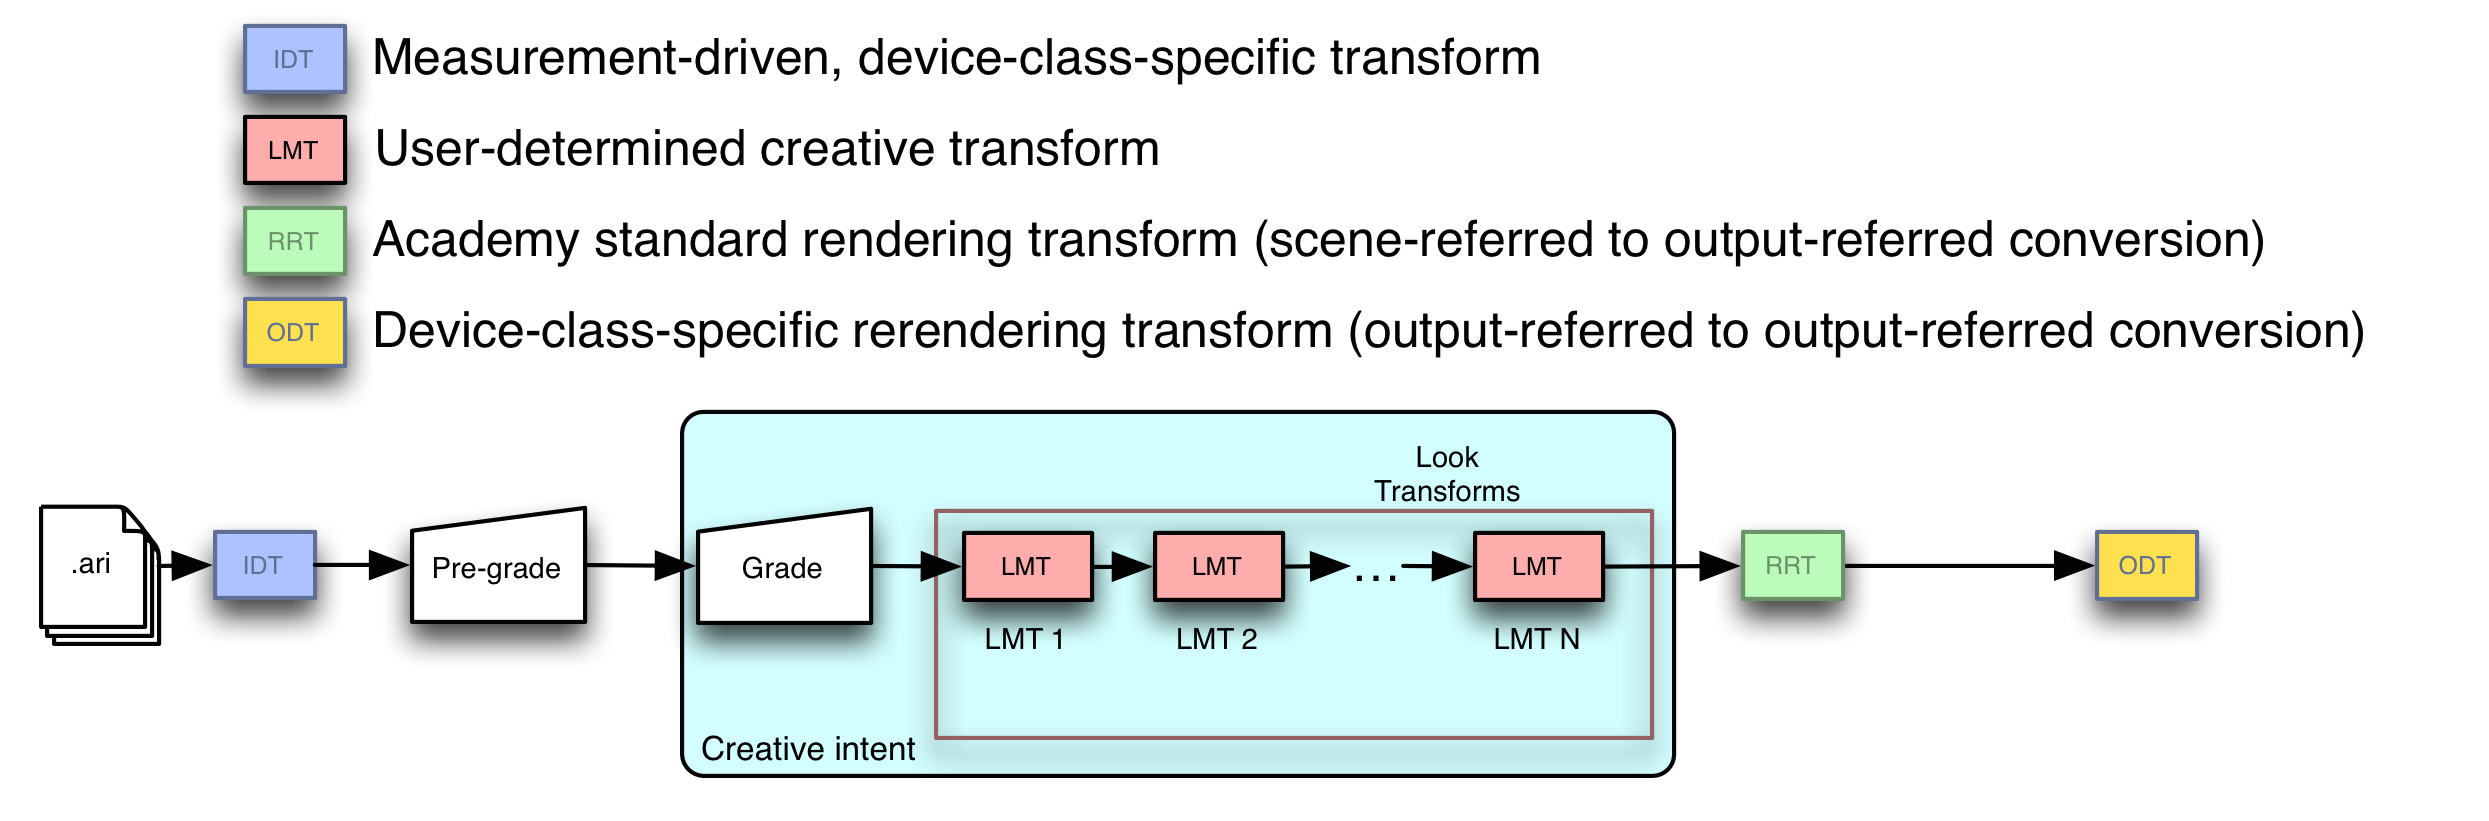
\includegraphics[width=\textwidth]{preview.png}
\caption{}
\label{fig:preview}
\end{center}
\end{figure}

The syntax and semantics of LMTs are given in the Specification section above. The syntax and semantics of pre-grading and grading operations are outside the scope of this document; indeed, they are outside the scope of the ACES project itself.

\section{Archival of ACES imagery with and without ‘baked in’ grading and/or LMT application}
Every archived ACES image has an implied associated displayed image, namely, the result of processing that archived ACES image with the RRT and the ODT that was used when creative approval was given. Because of this it is critical that the selected ODT (including all relevant versioning information) be archived alongside any archived ACES imagery, whether or not that ACES imagery is the product of `baking in' grades and/or the application of one or more LMTs making up a Look Transform.

Since many grading operations and LMTs may reduce the color volume in the original image to a smaller color volume that is then delivered to the RRT and a selected ODT, productions wishing to `future-proof' their assets should store the original ACES files, along with all pre-grading information, grading information, the ordered set of LMTs that make up the Look Transform and the ODT that was selected at the time of creative approval. (An LMT applying ASC CDL would be an example of such a color-volume-reducing transformation, as ASC CDL is applied in the ACEScc color space, a smaller color space than ACES.)
% This file contains the content for a main section
\regularsectionformat	% Change formatting to that of "Introduction" section
%% Modify below this line %%
\chapter{Design}

Simple LMTs are the best. An LMT should be as simple as possible while still achieving the desired modification to the displayed image.

\section{Overall principles}

\subsection{Support high dynamic range}
ACES image data can represent luminances from far below the detectability threshold of the human visual system all the way up to luminances causing physical pain — the maximum ACES luminance is about 65,505 times as bright as a diffuse white object in the scene. An LMT should endeavor to preserve this luminance range as much as is possible. 

\subsection{Handle a wide color gamut}
Creation of ACES imagery by CGI renderers, or by grading operations on live-action capture, can create ACES image values containing colors not found in nature—colors on the spectral locus that only became readily producible with the advent of the laser. An LMT should handle as wide a color gamut as is possible and practical, and avoid imposing arbitrary limits on hue or saturation. 

\subsection{Use high-level constructs to enable optimizations}
The Common LUT Format allows the ACES system release to provide a tool chest of predefined operations. LMT authors should use these rather than writing their own for several reasons:

\begin{itemize}
    \item   They were developed as part of the ACES project, have well-defined semantics, and are tested.
    \item   They obey the two principles above (‘Support high dynamic range’ and ‘Handle the full color gamut’) to the maximum extent possible,
    \item   Future releases might introduce performance or quality optimizations that depend on recognition of predefined operations.
\end{itemize}

\section{Analytic and empirical approaches}
Broadly speaking, LMTs can be characterized as either analytic or empirical. 

\subsection{Analytic LMTs}
Analytic LMTs usually have concise mathematical definitions. The prime example of an analytic LMT is probably the ACES-system-provided LMT that applies ASC CDL to ACES data. Another (hypothetical) analytic LMT might be one that changes saturation with luminance at certain hue angles. Analytic LMTs are typically expressed as a set of ordered mathematical operations or 1D LUT lookup operations on colors or color component values.

\subsection{Empirical LMTs}
Empirical LMTs usually are derived by sampling the results of some other color reproduction process, such as normal or special film processing. Empirical LMTs are often provided as 3D LUTs that record a regular subsampling of the results of such processes. 

A challenge arises when using ACES values to index the 3D LUT, as ACES values are radiometrically linear and have a very wide floating point range. The Common LUT Format provides for forward and inverse `shaper LUT' operations that (when wrapped around an appropriately constructed 3D LUT) effectively solve this problem. Implementers should review the `1D LUT' section of the Common LUT Format definition.

\section{Importing `looks' from non-ACES-color-managed workflows}
Importing a `look file' or LUT from a color system not defined using ACES can be quite difficult. Such ‘look files’ contain transforms to be applied in color spaces other than ACES or the ACES ‘working space’ used by ACESproxy and ACEScc, often presume the relationship between scene and encoded values is encoded with some (possibly proprietary) power function or log function, and likely are designed to supply a display device with code values directly rather than hand off the image to the RRT and a selected ODT.

For all of these reasons, it is typically better (and often much more efficient over the course of a production) to establish new Look Transforms within a workflow that is built around ACES-based color management rather than to try and mathematically translate a `look file' or LUT intended for use with a workflow based on some other color management system.

\begin{appendices}
    \appendixchapter{Example ACESclip File XML}{i}
\label{appendixA}

\begin{lstlisting}
<?xml version="1.0" encoding="UTF-8"?>
<aces:ACESmetadata xmlns:aces="http://www.oscars.org/aces/ref/acesmetadata">
<ContainerFormatVersion>1.0</ContainerFormatVersion>
<UUID type="urn:uuid:f81d4fae-7dec-11d0-a765-00a0c91e6bf6"/>
<ModificationTime>2014-11-24T10:20:13-8:00</ModificationTime>
<aces:Info>
    <Application version="2014">Vendor_ACESmaker v3</Application>
    <Comment>Day 1 Camera A: Indoors at Area 51</Comment>
</aces:Info>
<aces:ClipID>
    <ClipName>A0001B0003FX</ClipName>
    <Source_MediaID>A0001</Source_MediaID>
    <ClipDate>2014-11-20T12:24:13-8:00</ClipDate>
</aces:ClipID>
<aces:Config>
    <ACESrelease_Version>1.0</ACESrelease_Version>
    <Timestamp>2014-11-29T23:55:13-8:00</Timestamp>
    <aces:InputTransformList status="applied">
        <aces:IDTref TransformID="IDT.Sony.Slog2.v1">
            <LinkTransform>Slog2toACES.clf</LinkTransform>
        </aces:IDTref>
        <aces:GradeRef status="preview">
            <Convert_to_WorkSpace TransformID="ACEScsc.ACES_to_ACEScc.a1"/>
            <ColorDecisionList>
                <InputDescriptor>ACEScc</InputDescriptor>
                <ASC_CDL id="cc01234" inBitDepth="16f" outBitDepth="16f">
                    <SOPNode>
                        <Description>not a real example</Description>
                        <Slope>1.0000 1.0000 0.800000</Slope>
                        <Offset>0.0000 0.0000 0.000000</Offset>
                        <Power>1.0000 1.0000 1.000000</Power>
                    </SOPNode>
                    <SatNode>
                        <Saturation>0.9</Saturation>
                    </SatNode>
                </ASC_CDL>
            </ColorDecisionList>
            <Convert_from_WorkSpace { TransformID="ACEScc_to_ACES.a1"/>
        </aces:GradeRef>
        <LinkInputTransformList>F65presetgrade_seq4.clf</LinkInputTransformList>
    </aces:InputTransformList>
    <aces:PreviewTransformList status="preview">
        <aces:LMTref TransformID="LMT.Vendor.Locon.v1.ctl">
            <LinkTransform>f34d4fae-7dec-11d0-a765-00a0c91e6bf6</LinkTransform>
        </aces:LMTref>
            <aces:RRTref TransformID="RRT.Academy.a1"/>
        <aces:ODTref TransformID="ODT.Academy.Rec709_100nits_dim.a1">
            <LinkTransform>lut1023.clf</LinkTransform>
        </aces:ODTref>
        <LinkPreviewTransformList>V1_LMTlocon.clf</LinkPreviewTransformList>
    <aces:PreviewTransformList>
</aces:Config>

<aces:TransformLibrary>
    <ProcessList id="urn:uuid:f34d4fae-7dec-11d0-a765-00a0c91e6bf6">
        <Description>Sample 3DLUT for an LMT</Description>
        <InputDescriptor>ACES</InputDescriptor>
        <OutputDescriptor>ACES</OutputDescriptor>
        <LUT3D id="lmt_prodv2" name="LMT sequence 1 day exterior" 
                interpolation="tetrahedral" inBitDepth="16f" outBitDepth="12i">
            <Description>LMT Test File</Description>
            <Array dim="33 33 33 3">
                0    0    0
                1    1    1
                [...data omitted]
            </Array>
        </LUT3D>
    </ProcessList>
</aces:TransformLibrary>
</aces:ACESmetadata>
\end{lstlisting}

    \appendixchapter{Range of ACES values}{i}
\label{appendixB}

This appendix is intended for developers who wish to validate the accuracy of their implementation.

The table below contains the results of conversions using exact 16-bit ACES codes. 16-bit ACES has higher precision than either form of ACESproxy so rounding of ACES values will occur. These numbers are accurate for neutral values where R=G=B.

\begin{center}
\begin{tabularx}{\textwidth}{|Y|Y|Y|Y|Y|Y|}
\hline
\textbf{ACES 16-bit half-float Hex Code} & \textbf{ACES} & \textbf{ACESproxy 10-bit CV} & 
\textbf{ACESproxy 12-bit CV} & \textbf{ACES decoded from 10-bit ACESproxy} & \textbf{ACES decoded from 12-bit ACESproxy} \\ \hline
14DA & 0.001184464 & 64 & 256 & 0.001185417 & 0.001185417 \\ \hline
31C3 & 0.180053711 & 426 & 1705 & 0.179199219 & 0.179809570 \\ \hline
5AF7 & 222.875 & 940 & 3760 & 222.875 & 222.875 \\ \hline
\end{tabularx}
\end{center}
    
\end{appendices}

\end{document}